% Options for packages loaded elsewhere
\PassOptionsToPackage{unicode}{hyperref}
\PassOptionsToPackage{hyphens}{url}
%
\documentclass[
  oneside]{book}
\usepackage{amsmath,amssymb}
\usepackage{lmodern}
\usepackage{iftex}
\ifPDFTeX
  \usepackage[T1]{fontenc}
  \usepackage[utf8]{inputenc}
  \usepackage{textcomp} % provide euro and other symbols
\else % if luatex or xetex
  \usepackage{unicode-math}
  \defaultfontfeatures{Scale=MatchLowercase}
  \defaultfontfeatures[\rmfamily]{Ligatures=TeX,Scale=1}
\fi
% Use upquote if available, for straight quotes in verbatim environments
\IfFileExists{upquote.sty}{\usepackage{upquote}}{}
\IfFileExists{microtype.sty}{% use microtype if available
  \usepackage[]{microtype}
  \UseMicrotypeSet[protrusion]{basicmath} % disable protrusion for tt fonts
}{}
\makeatletter
\@ifundefined{KOMAClassName}{% if non-KOMA class
  \IfFileExists{parskip.sty}{%
    \usepackage{parskip}
  }{% else
    \setlength{\parindent}{0pt}
    \setlength{\parskip}{6pt plus 2pt minus 1pt}}
}{% if KOMA class
  \KOMAoptions{parskip=half}}
\makeatother
\usepackage{xcolor}
\IfFileExists{xurl.sty}{\usepackage{xurl}}{} % add URL line breaks if available
\IfFileExists{bookmark.sty}{\usepackage{bookmark}}{\usepackage{hyperref}}
\hypersetup{
  pdftitle={Microbiome data science with R/Bioconductor},
  hidelinks,
  pdfcreator={LaTeX via pandoc}}
\urlstyle{same} % disable monospaced font for URLs
\usepackage[top=30mm,left=15mm]{geometry}
\usepackage{color}
\usepackage{fancyvrb}
\newcommand{\VerbBar}{|}
\newcommand{\VERB}{\Verb[commandchars=\\\{\}]}
\DefineVerbatimEnvironment{Highlighting}{Verbatim}{commandchars=\\\{\}}
% Add ',fontsize=\small' for more characters per line
\usepackage{framed}
\definecolor{shadecolor}{RGB}{248,248,248}
\newenvironment{Shaded}{\begin{snugshade}}{\end{snugshade}}
\newcommand{\AlertTok}[1]{\textcolor[rgb]{0.94,0.16,0.16}{#1}}
\newcommand{\AnnotationTok}[1]{\textcolor[rgb]{0.56,0.35,0.01}{\textbf{\textit{#1}}}}
\newcommand{\AttributeTok}[1]{\textcolor[rgb]{0.77,0.63,0.00}{#1}}
\newcommand{\BaseNTok}[1]{\textcolor[rgb]{0.00,0.00,0.81}{#1}}
\newcommand{\BuiltInTok}[1]{#1}
\newcommand{\CharTok}[1]{\textcolor[rgb]{0.31,0.60,0.02}{#1}}
\newcommand{\CommentTok}[1]{\textcolor[rgb]{0.56,0.35,0.01}{\textit{#1}}}
\newcommand{\CommentVarTok}[1]{\textcolor[rgb]{0.56,0.35,0.01}{\textbf{\textit{#1}}}}
\newcommand{\ConstantTok}[1]{\textcolor[rgb]{0.00,0.00,0.00}{#1}}
\newcommand{\ControlFlowTok}[1]{\textcolor[rgb]{0.13,0.29,0.53}{\textbf{#1}}}
\newcommand{\DataTypeTok}[1]{\textcolor[rgb]{0.13,0.29,0.53}{#1}}
\newcommand{\DecValTok}[1]{\textcolor[rgb]{0.00,0.00,0.81}{#1}}
\newcommand{\DocumentationTok}[1]{\textcolor[rgb]{0.56,0.35,0.01}{\textbf{\textit{#1}}}}
\newcommand{\ErrorTok}[1]{\textcolor[rgb]{0.64,0.00,0.00}{\textbf{#1}}}
\newcommand{\ExtensionTok}[1]{#1}
\newcommand{\FloatTok}[1]{\textcolor[rgb]{0.00,0.00,0.81}{#1}}
\newcommand{\FunctionTok}[1]{\textcolor[rgb]{0.00,0.00,0.00}{#1}}
\newcommand{\ImportTok}[1]{#1}
\newcommand{\InformationTok}[1]{\textcolor[rgb]{0.56,0.35,0.01}{\textbf{\textit{#1}}}}
\newcommand{\KeywordTok}[1]{\textcolor[rgb]{0.13,0.29,0.53}{\textbf{#1}}}
\newcommand{\NormalTok}[1]{#1}
\newcommand{\OperatorTok}[1]{\textcolor[rgb]{0.81,0.36,0.00}{\textbf{#1}}}
\newcommand{\OtherTok}[1]{\textcolor[rgb]{0.56,0.35,0.01}{#1}}
\newcommand{\PreprocessorTok}[1]{\textcolor[rgb]{0.56,0.35,0.01}{\textit{#1}}}
\newcommand{\RegionMarkerTok}[1]{#1}
\newcommand{\SpecialCharTok}[1]{\textcolor[rgb]{0.00,0.00,0.00}{#1}}
\newcommand{\SpecialStringTok}[1]{\textcolor[rgb]{0.31,0.60,0.02}{#1}}
\newcommand{\StringTok}[1]{\textcolor[rgb]{0.31,0.60,0.02}{#1}}
\newcommand{\VariableTok}[1]{\textcolor[rgb]{0.00,0.00,0.00}{#1}}
\newcommand{\VerbatimStringTok}[1]{\textcolor[rgb]{0.31,0.60,0.02}{#1}}
\newcommand{\WarningTok}[1]{\textcolor[rgb]{0.56,0.35,0.01}{\textbf{\textit{#1}}}}
\usepackage{longtable,booktabs,array}
\usepackage{calc} % for calculating minipage widths
% Correct order of tables after \paragraph or \subparagraph
\usepackage{etoolbox}
\makeatletter
\patchcmd\longtable{\par}{\if@noskipsec\mbox{}\fi\par}{}{}
\makeatother
% Allow footnotes in longtable head/foot
\IfFileExists{footnotehyper.sty}{\usepackage{footnotehyper}}{\usepackage{footnote}}
\makesavenoteenv{longtable}
\usepackage{graphicx}
\makeatletter
\def\maxwidth{\ifdim\Gin@nat@width>\linewidth\linewidth\else\Gin@nat@width\fi}
\def\maxheight{\ifdim\Gin@nat@height>\textheight\textheight\else\Gin@nat@height\fi}
\makeatother
% Scale images if necessary, so that they will not overflow the page
% margins by default, and it is still possible to overwrite the defaults
% using explicit options in \includegraphics[width, height, ...]{}
\setkeys{Gin}{width=\maxwidth,height=\maxheight,keepaspectratio}
% Set default figure placement to htbp
\makeatletter
\def\fps@figure{htbp}
\makeatother
\setlength{\emergencystretch}{3em} % prevent overfull lines
\providecommand{\tightlist}{%
  \setlength{\itemsep}{0pt}\setlength{\parskip}{0pt}}
\setcounter{secnumdepth}{5}
\usepackage{booktabs}
\ifLuaTeX
  \usepackage{selnolig}  % disable illegal ligatures
\fi
\usepackage[]{natbib}
\bibliographystyle{apalike}

\title{Microbiome data science with R/Bioconductor}
\usepackage{etoolbox}
\makeatletter
\providecommand{\subtitle}[1]{% add subtitle to \maketitle
  \apptocmd{\@title}{\par {\large #1 \par}}{}{}
}
\makeatother
\subtitle{Welcome to Radboud Summer School, July 2022}
\author{}
\date{\vspace{-2.5em}2022-07-06}

\begin{document}
\maketitle

{
\setcounter{tocdepth}{1}
\tableofcontents
}
\hypertarget{overview}{%
\chapter{Overview}\label{overview}}

\hypertarget{contents-and-learning-goals}{%
\section{Contents and learning goals}\label{contents-and-learning-goals}}

This course will focus on \textbf{microbiome data analysis
with R/Bioconductor}, a popular open source environment for
scientific data analysis. You will get an overview of the
reproducible data analysis workflows in microbiome research, with a
focus on gut-brain axis studies.

After the course you will know how to approach new tasks in the
analysis of taxonomic profiling data by taking advantage of available
documentation and R tools.

The teaching follows the open online documentation created by the
course teachers, extending the online book Orchestrating Microbiome
Analysis (\url{https://microbiome.github.io/OMA}). The openly licensed
teaching material will be available online during and after the
course, following Finnish national recommendations on open education.

The training material walks you through the standard steps of
biomedical data analysis covering data access, exploration, analysis,
visualization, reproducible reporting, and best practices in open
science. We will teach generic data analytical skills that are
applicable to common data analysis tasks encountered in modern omics
research. The teaching format allows adaptations according to the
student's learning speed.

\hypertarget{schedule-and-organizers}{%
\section{Schedule and organizers}\label{schedule-and-organizers}}

\textbf{Format} In-person course. For detailed schedule, see the
\href{https://www.ru.nl/radboudsummerschool/courses/2022/registration-longer-possible-brain-bacteria}{course
website}.

\textbf{Venue} University of Radboud. July 11-15, 2022.

\textbf{Expected background}

\textbf{Target audience} The course is primarily designed for advanced MSc
and PhD students, Postdocs, and biomedical researchers who wish to
learn new skills in scientific programming and biomedical data
analysis. Academic students and researchers encouraged to
apply. Priority will be given for local students. Some earlier
experience with R or another programming language is recommended.

\textbf{Preparation} Advance preparation is expected. Online support is available. See section \ref{start} for instructions.

\hypertarget{acknowledgments}{%
\section{Acknowledgments}\label{acknowledgments}}

\textbf{Citation} We thank all \href{https://microbiome.github.io}{developers and contributors} who have contributed open resources that supported the development of the training material. Kindly cite the course material as \citet{radboud2022course}

\textbf{Contact} See \url{https://microbiome.github.io}

\textbf{License and source code}

All material is released under the open \href{LICENSE}{CC BY-NC-SA 3.0
License} and available online during and after the course,
following the \href{https://avointiede.fi/fi/linjaukset-ja-aineistot/kotimaiset-linjaukset/oppimisen-ja-oppimateriaalien-avoimuuden-linjaus}{recommendations on open teaching
materials}
of the national open science coordination in Finland. The source code
of this repository is reproducible and contains the Rmd files with
executable code. See \href{README.md}{README}.

\hypertarget{code-of-conduct}{%
\chapter{Code of Conduct}\label{code-of-conduct}}

The Bioconductor community values an open approach to science that promotes the

\begin{itemize}
\tightlist
\item
  sharing of ideas, code, software and expertise
\item
  collaboration
\item
  diversity and inclusivity
\item
  a kind and welcoming environment
\item
  community contributions
\end{itemize}

We value your attendance and participation at Bioconductor events and in our community.

For the full version, enforcement, and reporting instructions, see the \href{https://bioconductor.github.io/bioc_coc_multilingual/}{Bioconductor code of conduct}.

\hypertarget{start}{%
\chapter{Getting started}\label{start}}

\hypertarget{checklist-before-the-course}{%
\section{Checklist (before the course)}\label{checklist-before-the-course}}

\hypertarget{computer-setup-and-installations}{%
\subsection{Computer setup and installations}\label{computer-setup-and-installations}}

Setting up the system on your own computer is not required for the
course but it can be useful for later use. The required software:

\begin{itemize}
\item
  \href{https://www.r-project.org/}{R (version \textgreater4.2.0)}
\item
  \href{https://www.rstudio.com/products/rstudio/download/}{RStudio};
  choose ``Rstudio Desktop'' to download the latest version. Optional
  but preferred. For further details, check the \href{https://www.rstudio.com/}{Rstudio home
  page}.
\item
  Install and load the required R packages (see Section \ref{packages})
\item
  After a successful installation you can start with the
  case study examples in this training material
\end{itemize}

\hypertarget{support-and-resources}{%
\section{Support and resources}\label{support-and-resources}}

\begin{itemize}
\item
  We recommend to have a look at the additional reading tips and try out online material listed in Section \ref{material}.
\item
  \textbf{You can run the workflows by simply copy-pasting the examples.}
  For further, advanced material, you can test and modify further
  examples from the online book, and apply these techniques to your own
  data.
\item
  Online support on installation and other matters, join us at \href{https://gitter.im/microbiome/miaverse?utm_source=badge\&utm_medium=badge\&utm_campaign=pr-badge\&utm_content=badge}{Gitter}
\end{itemize}

\hypertarget{packages}{%
\section{Installing and loading the required R packages}\label{packages}}

You may need the examples from this subsection if you are installing
the environment on your own computer. If you need to add new packages,
you can modify the examples below.

This section shows how to install and load all required packages into
the R session, if needed. Only uninstalled packages are installed.

Download the file \url{pkgs.csv}. This contains the list of
packages that we recommend to preinstall. This can be done with the
following code.

\begin{Shaded}
\begin{Highlighting}[]
\CommentTok{\# List of packages that we need}
\NormalTok{pkg }\OtherTok{\textless{}{-}} \FunctionTok{read.csv}\NormalTok{(}\StringTok{"pkgs.csv"}\NormalTok{)[,}\DecValTok{1}\NormalTok{]}

\CommentTok{\# List packages that are already installed}
\NormalTok{pkg\_already\_installed }\OtherTok{\textless{}{-}}\NormalTok{ pkg[ pkg }\SpecialCharTok{\%in\%} \FunctionTok{installed.packages}\NormalTok{() ]}

\CommentTok{\# List remaining packages that need to be installed}
\NormalTok{packages\_to\_install }\OtherTok{\textless{}{-}} \FunctionTok{setdiff}\NormalTok{(pkg, pkg\_already\_installed)}
\end{Highlighting}
\end{Shaded}

\begin{Shaded}
\begin{Highlighting}[]
\CommentTok{\# If there are packages that need to be installed, install them }
\ControlFlowTok{if}\NormalTok{( }\FunctionTok{length}\NormalTok{(packages\_to\_install) ) \{}
\NormalTok{   BiocManager}\SpecialCharTok{::}\FunctionTok{install}\NormalTok{(packages\_to\_install)}
\NormalTok{\}}
\end{Highlighting}
\end{Shaded}

Now all required packages are installed, so let's load them into the session.
Some function names occur in multiple packages. That is why miaverse's packages
mia and miaViz are prioritized. Packages that are loaded first have higher priority.

\begin{Shaded}
\begin{Highlighting}[]
\CommentTok{\# Loading all packages into session. Returns true if package was successfully loaded.}
\NormalTok{loaded }\OtherTok{\textless{}{-}} \FunctionTok{sapply}\NormalTok{(packages, require, }\AttributeTok{character.only =} \ConstantTok{TRUE}\NormalTok{)}
\FunctionTok{as.data.frame}\NormalTok{(loaded)}
\end{Highlighting}
\end{Shaded}

\hypertarget{importing-microbiome-data}{%
\chapter{Importing microbiome data}\label{importing-microbiome-data}}

This section demonstrates how to import microbiome profiling data in R.

\hypertarget{data-access}{%
\section{Data access}\label{data-access}}

\textbf{Option 1}

\emph{ADHD-associated changes in gut microbiota and brain in a mouse model}

Tengeler AC \emph{et
al.} (2020) \href{https://doi.org/10.1186/s40168-020-00816-x}{\textbf{Gut microbiota from persons with
attention-deficit/hyperactivity disorder affects the brain in
mice}}. Microbiome
8:44.

In this study, mice are colonized with microbiota from participants
with ADHD (attention deficit hyperactivity disorder) and healthy
participants. The aim of the study was to assess whether the mice
display ADHD behaviors after being inoculated with ADHD microbiota,
suggesting a role of the microbiome in ADHD pathology.

Download the data from
\href{https://github.com/microbiome/course_2022_radboud/tree/main/data}{data}
subfolder.

\textbf{Option 2}

\emph{Open data set of your own choice}, different options are listed in \href{https://microbiome.github.io/OMA/containers.html\#example-data}{OMA}.

\hypertarget{importing-microbiome-data-in-r}{%
\section{Importing microbiome data in R}\label{importing-microbiome-data-in-r}}

\textbf{Import example data} by modifying the examples in the online book
section on \href{https://microbiome.github.io/OMA/data-introduction.html\#loading-experimental-microbiome-data}{data exploration and
manipulation}. The
data files in our example are in \emph{biom} format, which is a standard
file format for microbiome data. Other file formats exist as well, and
import details vary by platform.

Here, we import \emph{biom} data files into a specific data container (structure)
in R, \emph{TreeSummarizedExperiment} (TSE) \href{https://f1000research.com/articles/9-1246}{Huang et
al.~(2020)}. This provides
the basis for downstream data analysis in the \emph{miaverse} data science
framework.

In this course, we focus on downstream analysis of taxonomic profiling
data, and assume that the data has already been appropriately
preprocessed and available in the TSE format. In addition to our
example data, further demonstration data sets are readily available in
the TSE format through
\href{https://bioconductor.org/packages/release/data/experiment/html/microbiomeDataSets.html}{microbiomeDataSets}.

\textbf{Figure sources:}

\textbf{Original article}
- Huang R \emph{et al}. (2021) \href{https://doi.org/10.12688/\%20f1000research.26669.2}{TreeSummarizedExperiment: a S4 class
for data with hierarchical structure}. F1000Research 9:1246.

\textbf{Reference Sequence slot extension}
- Lahti L \emph{et al}. (2020) \href{https://doi.org/10.7490/\%20f1000research.1118447.1}{Upgrading the R/Bioconductor ecosystem for microbiome
research} F1000Research 9:1464 (slides).

\hypertarget{example-solutions}{%
\section{Example solutions}\label{example-solutions}}

\begin{itemize}
\tightlist
\item
  Example code for data import: \url{import.Rmd}
\end{itemize}

\hypertarget{reproducible-reporting-with-rmarkdown}{%
\chapter{Reproducible reporting with Rmarkdown}\label{reproducible-reporting-with-rmarkdown}}

Reproducible reporting is the starting point for robust interactive
data science. Perform the following tasks:

\begin{itemize}
\item
  If you are entirely new to Markdown, take
  \href{https://www.markdowntutorial.com/}{this} 10 minute tutorial to get
  introduced to the most important functions within Markdown. Then
  experiment with different options with
  \href{https://www.rstudio.com/wp-content/uploads/2015/02/rmarkdown-cheatsheet.pdf}{Rmarkdown}
\item
  Create a Rmarkdown template in RStudio, and render it into a
  document (markdown, PDF, docx or other format). In case you are new
  to Rmarkdown \href{https://rmarkdown.rstudio.com/lesson-1.html}{Rstudio provides
  resources} to learn
  about the use cases and the basics of Rmarkdown.
\item
  Further examples are tips for Rmarkdown are available in the
  online tutorial to reproducible reporting by \href{https://rpubs.com/marschmi/RMarkdown}{Dr.~C Titus
  Brown}.
\end{itemize}

\hypertarget{material}{%
\chapter{Study material}\label{material}}

\hypertarget{online-tutorial}{%
\section{Online tutorial}\label{online-tutorial}}

The course will utilize material from the online book (beta version)
\href{https://microbiome.github.io/OMA/}{Orchestrating Microbiome Analysis with R/Bioconductor
(OMA)}. We encourage to familiarize
with this material and test examples already before the course.

\hypertarget{lecture-slides}{%
\section{Lecture slides}\label{lecture-slides}}

To be added.

\hypertarget{tasks}{%
\section{Tasks}\label{tasks}}

Seek guidance from the \url{https://microbiome.github.io/OMA/}

\begin{itemize}
\item
  \href{https://microbiome.github.io/OMA/exercises.html}{Exercises}
\item
  \href{https://github.com/microbiome/course_2022_radboud/blob/main/example_solutions.Rmd}{Example solutions}
\end{itemize}

\hypertarget{extra-material-on-miaverse-and-r-programming}{%
\section{Extra material on miaverse and R programming}\label{extra-material-on-miaverse-and-r-programming}}

\href{https://microbiome.github.io/OMA/resources.html}{Further information on the data science framework}

\hypertarget{alpha-diversity-demo}{%
\chapter{Alpha diversity demo}\label{alpha-diversity-demo}}

\hypertarget{alpha-diversity-estimation}{%
\section{Alpha diversity estimation}\label{alpha-diversity-estimation}}

First let`s load the required packages and data set

\begin{Shaded}
\begin{Highlighting}[]
\FunctionTok{library}\NormalTok{(mia)}
\end{Highlighting}
\end{Shaded}

\begin{verbatim}
## Loading required package: SummarizedExperiment
\end{verbatim}

\begin{verbatim}
## Loading required package: MatrixGenerics
\end{verbatim}

\begin{verbatim}
## Loading required package: matrixStats
\end{verbatim}

\begin{verbatim}
## 
## Attaching package: 'MatrixGenerics'
\end{verbatim}

\begin{verbatim}
## The following objects are masked from 'package:matrixStats':
## 
##     colAlls, colAnyNAs, colAnys, colAvgsPerRowSet, colCollapse,
##     colCounts, colCummaxs, colCummins, colCumprods, colCumsums,
##     colDiffs, colIQRDiffs, colIQRs, colLogSumExps, colMadDiffs,
##     colMads, colMaxs, colMeans2, colMedians, colMins, colOrderStats,
##     colProds, colQuantiles, colRanges, colRanks, colSdDiffs, colSds,
##     colSums2, colTabulates, colVarDiffs, colVars, colWeightedMads,
##     colWeightedMeans, colWeightedMedians, colWeightedSds,
##     colWeightedVars, rowAlls, rowAnyNAs, rowAnys, rowAvgsPerColSet,
##     rowCollapse, rowCounts, rowCummaxs, rowCummins, rowCumprods,
##     rowCumsums, rowDiffs, rowIQRDiffs, rowIQRs, rowLogSumExps,
##     rowMadDiffs, rowMads, rowMaxs, rowMeans2, rowMedians, rowMins,
##     rowOrderStats, rowProds, rowQuantiles, rowRanges, rowRanks,
##     rowSdDiffs, rowSds, rowSums2, rowTabulates, rowVarDiffs, rowVars,
##     rowWeightedMads, rowWeightedMeans, rowWeightedMedians,
##     rowWeightedSds, rowWeightedVars
\end{verbatim}

\begin{verbatim}
## Loading required package: GenomicRanges
\end{verbatim}

\begin{verbatim}
## Loading required package: stats4
\end{verbatim}

\begin{verbatim}
## Loading required package: BiocGenerics
\end{verbatim}

\begin{verbatim}
## 
## Attaching package: 'BiocGenerics'
\end{verbatim}

\begin{verbatim}
## The following objects are masked from 'package:stats':
## 
##     IQR, mad, sd, var, xtabs
\end{verbatim}

\begin{verbatim}
## The following objects are masked from 'package:base':
## 
##     anyDuplicated, append, as.data.frame, basename, cbind, colnames,
##     dirname, do.call, duplicated, eval, evalq, Filter, Find, get, grep,
##     grepl, intersect, is.unsorted, lapply, Map, mapply, match, mget,
##     order, paste, pmax, pmax.int, pmin, pmin.int, Position, rank,
##     rbind, Reduce, rownames, sapply, setdiff, sort, table, tapply,
##     union, unique, unsplit, which.max, which.min
\end{verbatim}

\begin{verbatim}
## Loading required package: S4Vectors
\end{verbatim}

\begin{verbatim}
## 
## Attaching package: 'S4Vectors'
\end{verbatim}

\begin{verbatim}
## The following objects are masked from 'package:base':
## 
##     expand.grid, I, unname
\end{verbatim}

\begin{verbatim}
## Loading required package: IRanges
\end{verbatim}

\begin{verbatim}
## Loading required package: GenomeInfoDb
\end{verbatim}

\begin{verbatim}
## Loading required package: Biobase
\end{verbatim}

\begin{verbatim}
## Welcome to Bioconductor
## 
##     Vignettes contain introductory material; view with
##     'browseVignettes()'. To cite Bioconductor, see
##     'citation("Biobase")', and for packages 'citation("pkgname")'.
\end{verbatim}

\begin{verbatim}
## 
## Attaching package: 'Biobase'
\end{verbatim}

\begin{verbatim}
## The following object is masked from 'package:MatrixGenerics':
## 
##     rowMedians
\end{verbatim}

\begin{verbatim}
## The following objects are masked from 'package:matrixStats':
## 
##     anyMissing, rowMedians
\end{verbatim}

\begin{verbatim}
## Loading required package: SingleCellExperiment
\end{verbatim}

\begin{verbatim}
## Loading required package: TreeSummarizedExperiment
\end{verbatim}

\begin{verbatim}
## Loading required package: Biostrings
\end{verbatim}

\begin{verbatim}
## Loading required package: XVector
\end{verbatim}

\begin{verbatim}
## 
## Attaching package: 'Biostrings'
\end{verbatim}

\begin{verbatim}
## The following object is masked from 'package:base':
## 
##     strsplit
\end{verbatim}

\begin{verbatim}
## Loading required package: MultiAssayExperiment
\end{verbatim}

\begin{Shaded}
\begin{Highlighting}[]
\FunctionTok{library}\NormalTok{(miaViz)}
\end{Highlighting}
\end{Shaded}

\begin{verbatim}
## Loading required package: ggplot2
\end{verbatim}

\begin{verbatim}
## Loading required package: ggraph
\end{verbatim}

\begin{Shaded}
\begin{Highlighting}[]
\FunctionTok{library}\NormalTok{(tidyverse)}
\end{Highlighting}
\end{Shaded}

\begin{verbatim}
## -- Attaching packages --------------------------------------- tidyverse 1.3.1 --
\end{verbatim}

\begin{verbatim}
## v tibble  3.1.7     v dplyr   1.0.9
## v tidyr   1.2.0     v stringr 1.4.0
## v readr   2.1.2     v forcats 0.5.1
## v purrr   0.3.4
\end{verbatim}

\begin{verbatim}
## -- Conflicts ------------------------------------------ tidyverse_conflicts() --
## x dplyr::collapse()   masks Biostrings::collapse(), IRanges::collapse()
## x dplyr::combine()    masks Biobase::combine(), BiocGenerics::combine()
## x purrr::compact()    masks XVector::compact()
## x dplyr::count()      masks matrixStats::count()
## x dplyr::desc()       masks IRanges::desc()
## x tidyr::expand()     masks S4Vectors::expand()
## x dplyr::filter()     masks stats::filter()
## x dplyr::first()      masks S4Vectors::first()
## x dplyr::lag()        masks stats::lag()
## x ggplot2::Position() masks BiocGenerics::Position(), base::Position()
## x purrr::reduce()     masks GenomicRanges::reduce(), IRanges::reduce()
## x dplyr::rename()     masks S4Vectors::rename()
## x dplyr::slice()      masks XVector::slice(), IRanges::slice()
\end{verbatim}

\begin{Shaded}
\begin{Highlighting}[]
\CommentTok{\# library(vegan)}

\NormalTok{tse }\OtherTok{\textless{}{-}} \FunctionTok{read\_rds}\NormalTok{(}\StringTok{"data/Tengeler2020/tse.rds"}\NormalTok{)}

\NormalTok{tse}
\end{Highlighting}
\end{Shaded}

\begin{verbatim}
## class: TreeSummarizedExperiment 
## dim: 151 27 
## metadata(0):
## assays(1): counts
## rownames(151): 1726470 1726471 ... 17264756 17264757
## rowData names(6): Kingdom Phylum ... Family Genus
## colnames(27): A110 A12 ... A35 A38
## colData names(4): patient_status cohort patient_status_vs_cohort
##   sample_name
## reducedDimNames(0):
## mainExpName: NULL
## altExpNames(0):
## rowLinks: a LinkDataFrame (151 rows)
## rowTree: 1 phylo tree(s) (151 leaves)
## colLinks: NULL
## colTree: NULL
\end{verbatim}

Then let's estimate multiple diversity indices.

\begin{Shaded}
\begin{Highlighting}[]
\NormalTok{?estimateDiversity}

\NormalTok{tse }\OtherTok{\textless{}{-}} \FunctionTok{estimateDiversity}\NormalTok{(tse, }
                              \AttributeTok{index =} \FunctionTok{c}\NormalTok{(}\StringTok{"shannon"}\NormalTok{,}\StringTok{"gini\_simpson"}\NormalTok{,}\StringTok{"faith"}\NormalTok{),}
                              \AttributeTok{name =} \FunctionTok{c}\NormalTok{(}\StringTok{"shannon"}\NormalTok{,}\StringTok{"gini\_simpson"}\NormalTok{,}\StringTok{"faith"}\NormalTok{))}
\FunctionTok{head}\NormalTok{(}\FunctionTok{colData}\NormalTok{(tse))}
\end{Highlighting}
\end{Shaded}

\begin{verbatim}
## DataFrame with 6 rows and 7 columns
##      patient_status      cohort patient_status_vs_cohort sample_name   shannon
##         <character> <character>              <character> <character> <numeric>
## A110           ADHD    Cohort_1            ADHD_Cohort_1        A110   1.76541
## A12            ADHD    Cohort_1            ADHD_Cohort_1         A12   2.71644
## A15            ADHD    Cohort_1            ADHD_Cohort_1         A15   3.17810
## A19            ADHD    Cohort_1            ADHD_Cohort_1         A19   2.89199
## A21            ADHD    Cohort_2            ADHD_Cohort_2         A21   2.84198
## A23            ADHD    Cohort_2            ADHD_Cohort_2         A23   2.79794
##      gini_simpson     faith
##         <numeric> <numeric>
## A110     0.669537   7.39224
## A12      0.871176   6.29378
## A15      0.930561   6.60608
## A19      0.899210   6.79708
## A21      0.885042   6.65110
## A23      0.859813   5.96246
\end{verbatim}

We can see that the variables are included in the data.
Similarly, let's calculate richness indices.

\begin{Shaded}
\begin{Highlighting}[]
\NormalTok{tse }\OtherTok{\textless{}{-}} \FunctionTok{estimateRichness}\NormalTok{(tse, }
                              \AttributeTok{index =} \FunctionTok{c}\NormalTok{(}\StringTok{"chao1"}\NormalTok{,}\StringTok{"observed"}\NormalTok{))}
\FunctionTok{head}\NormalTok{(}\FunctionTok{colData}\NormalTok{(tse))}
\end{Highlighting}
\end{Shaded}

\begin{verbatim}
## DataFrame with 6 rows and 10 columns
##      patient_status      cohort patient_status_vs_cohort sample_name   shannon
##         <character> <character>              <character> <character> <numeric>
## A110           ADHD    Cohort_1            ADHD_Cohort_1        A110   1.76541
## A12            ADHD    Cohort_1            ADHD_Cohort_1         A12   2.71644
## A15            ADHD    Cohort_1            ADHD_Cohort_1         A15   3.17810
## A19            ADHD    Cohort_1            ADHD_Cohort_1         A19   2.89199
## A21            ADHD    Cohort_2            ADHD_Cohort_2         A21   2.84198
## A23            ADHD    Cohort_2            ADHD_Cohort_2         A23   2.79794
##      gini_simpson     faith     chao1  chao1_se  observed
##         <numeric> <numeric> <numeric> <numeric> <numeric>
## A110     0.669537   7.39224        68  0.000000        68
## A12      0.871176   6.29378        51  0.000000        51
## A15      0.930561   6.60608        68  0.000000        68
## A19      0.899210   6.79708        62  0.000000        62
## A21      0.885042   6.65110        58  0.000000        58
## A23      0.859813   5.96246        61  0.247942        61
\end{verbatim}

\hypertarget{visualizing-alpha-diversity}{%
\section{Visualizing alpha diversity}\label{visualizing-alpha-diversity}}

We can plot the distributions of individual indices:

\begin{Shaded}
\begin{Highlighting}[]
\CommentTok{\#individual plot}
\NormalTok{p }\OtherTok{\textless{}{-}} \FunctionTok{as\_tibble}\NormalTok{(}\FunctionTok{colData}\NormalTok{(tse)) }\SpecialCharTok{\%\textgreater{}\%} 
  \FunctionTok{ggplot}\NormalTok{(}\FunctionTok{aes}\NormalTok{(shannon)) }\SpecialCharTok{+}
  \FunctionTok{geom\_histogram}\NormalTok{() }

\FunctionTok{print}\NormalTok{(p)}
\end{Highlighting}
\end{Shaded}

\begin{verbatim}
## `stat_bin()` using `bins = 30`. Pick better value with `binwidth`.
\end{verbatim}

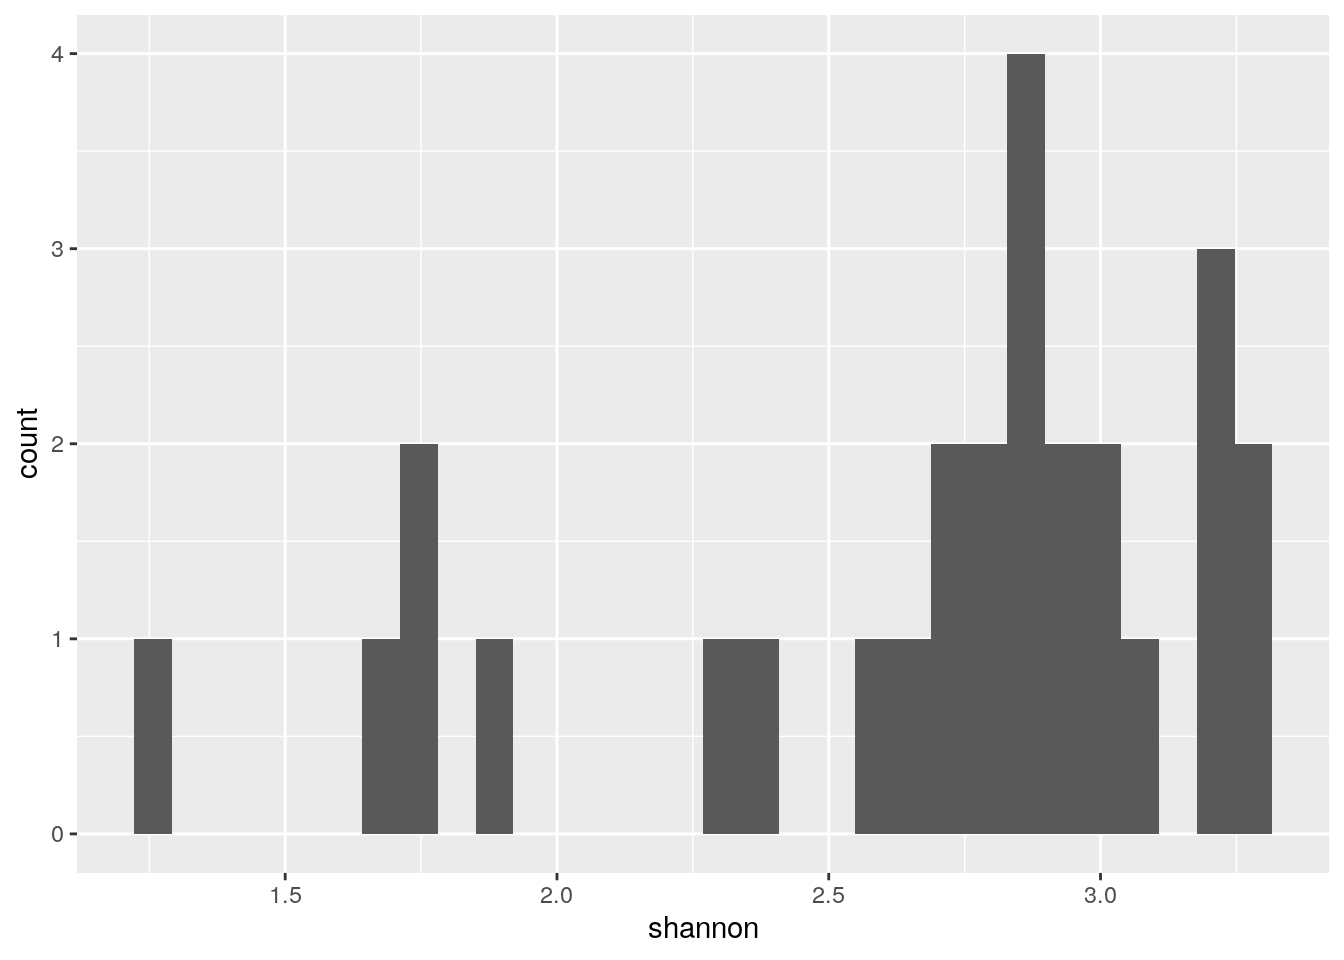
\includegraphics{05-alpha_diversity_demo_files/figure-latex/distributions-1.pdf}

\begin{Shaded}
\begin{Highlighting}[]
\CommentTok{\#multiple plots}

\NormalTok{p }\OtherTok{\textless{}{-}} \FunctionTok{as\_tibble}\NormalTok{(}\FunctionTok{colData}\NormalTok{(tse)) }\SpecialCharTok{\%\textgreater{}\%} 
  \FunctionTok{pivot\_longer}\NormalTok{(}\AttributeTok{cols =} \FunctionTok{c}\NormalTok{(}\StringTok{"shannon"}\NormalTok{,}\StringTok{"gini\_simpson"}\NormalTok{,}\StringTok{"faith"}\NormalTok{,}\StringTok{"chao1"}\NormalTok{,}\StringTok{"observed"}\NormalTok{), }\AttributeTok{names\_to =} \StringTok{"index"}\NormalTok{, }\AttributeTok{values\_to =} \StringTok{"alpha"}\NormalTok{) }\SpecialCharTok{\%\textgreater{}\%} 
  \FunctionTok{ggplot}\NormalTok{(}\FunctionTok{aes}\NormalTok{(alpha)) }\SpecialCharTok{+}
  \FunctionTok{geom\_histogram}\NormalTok{() }\SpecialCharTok{+}
  \FunctionTok{facet\_wrap}\NormalTok{(}\FunctionTok{vars}\NormalTok{(index), }\AttributeTok{scales =} \StringTok{"free"}\NormalTok{)}


\FunctionTok{print}\NormalTok{(p)}
\end{Highlighting}
\end{Shaded}

\begin{verbatim}
## `stat_bin()` using `bins = 30`. Pick better value with `binwidth`.
\end{verbatim}

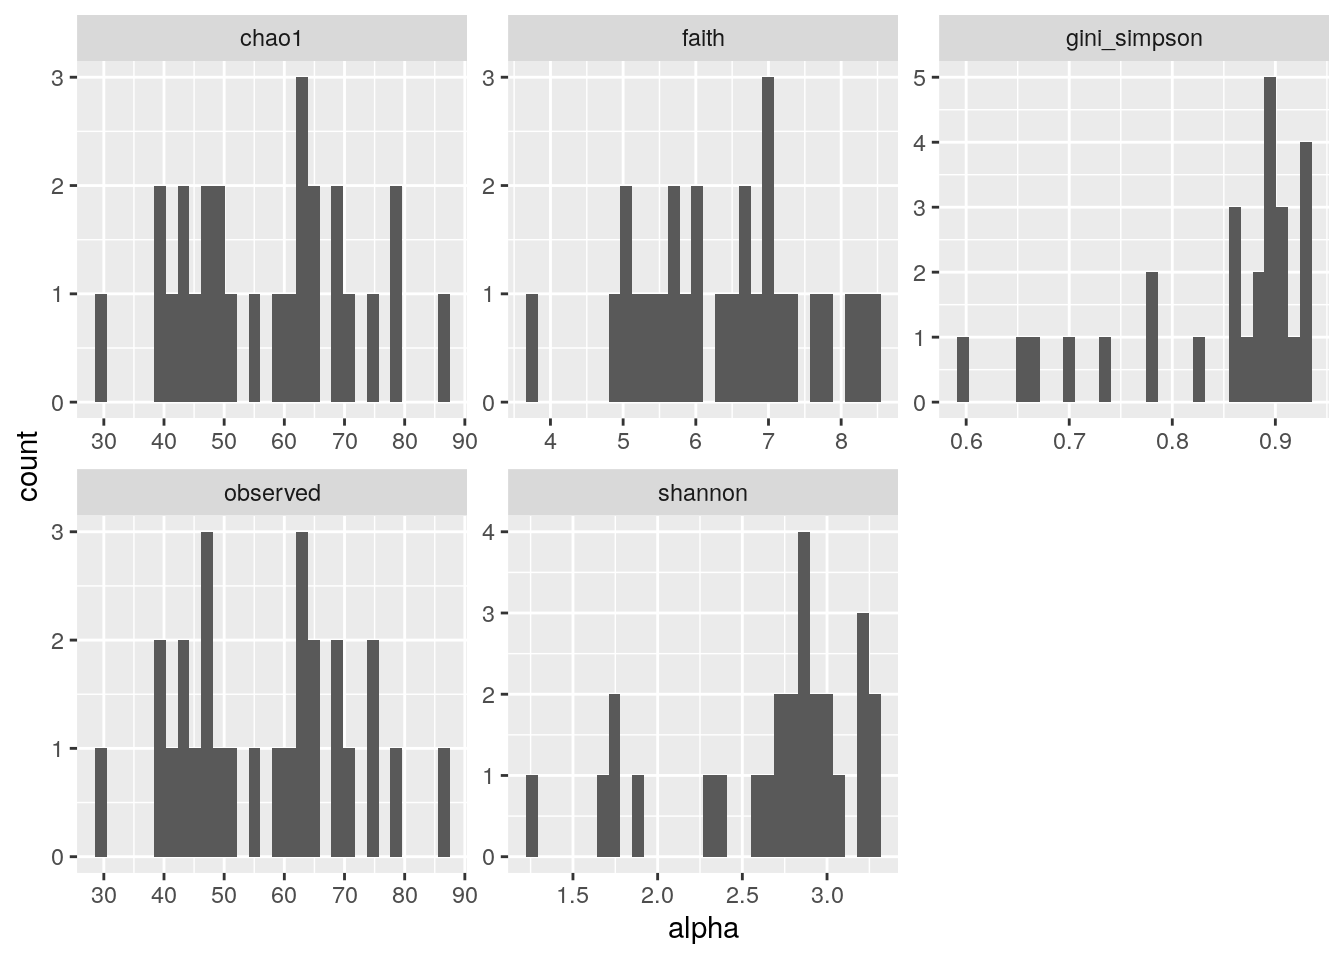
\includegraphics{05-alpha_diversity_demo_files/figure-latex/distributions-2.pdf}

and the correlation between indices:

\begin{Shaded}
\begin{Highlighting}[]
\NormalTok{p }\OtherTok{\textless{}{-}} \FunctionTok{as\_tibble}\NormalTok{(}\FunctionTok{colData}\NormalTok{(tse)) }\SpecialCharTok{\%\textgreater{}\%} 
  \FunctionTok{pivot\_longer}\NormalTok{(}\AttributeTok{cols =} \FunctionTok{c}\NormalTok{(}\StringTok{"shannon"}\NormalTok{,}\StringTok{"gini\_simpson"}\NormalTok{,}\StringTok{"faith"}\NormalTok{,}\StringTok{"chao1"}\NormalTok{,}\StringTok{"observed"}\NormalTok{), }\AttributeTok{names\_to =} \StringTok{"index"}\NormalTok{, }\AttributeTok{values\_to =} \StringTok{"alpha"}\NormalTok{) }\SpecialCharTok{\%\textgreater{}\%} 
  \FunctionTok{full\_join}\NormalTok{(.,., }\AttributeTok{by =} \StringTok{"sample\_name"}\NormalTok{) }\SpecialCharTok{\%\textgreater{}\%} 
  \FunctionTok{ggplot}\NormalTok{( }\FunctionTok{aes}\NormalTok{(}\AttributeTok{x =}\NormalTok{ alpha.x, }\AttributeTok{y =}\NormalTok{ alpha.y)) }\SpecialCharTok{+} 
  \FunctionTok{geom\_point}\NormalTok{() }\SpecialCharTok{+}
  \FunctionTok{geom\_smooth}\NormalTok{() }\SpecialCharTok{+}
  \FunctionTok{facet\_wrap}\NormalTok{(index.x }\SpecialCharTok{\textasciitilde{}}\NormalTok{ index.y, }\AttributeTok{scales =} \StringTok{"free"}\NormalTok{)}

\FunctionTok{print}\NormalTok{(p)}
\end{Highlighting}
\end{Shaded}

\begin{verbatim}
## `geom_smooth()` using method = 'loess' and formula 'y ~ x'
\end{verbatim}

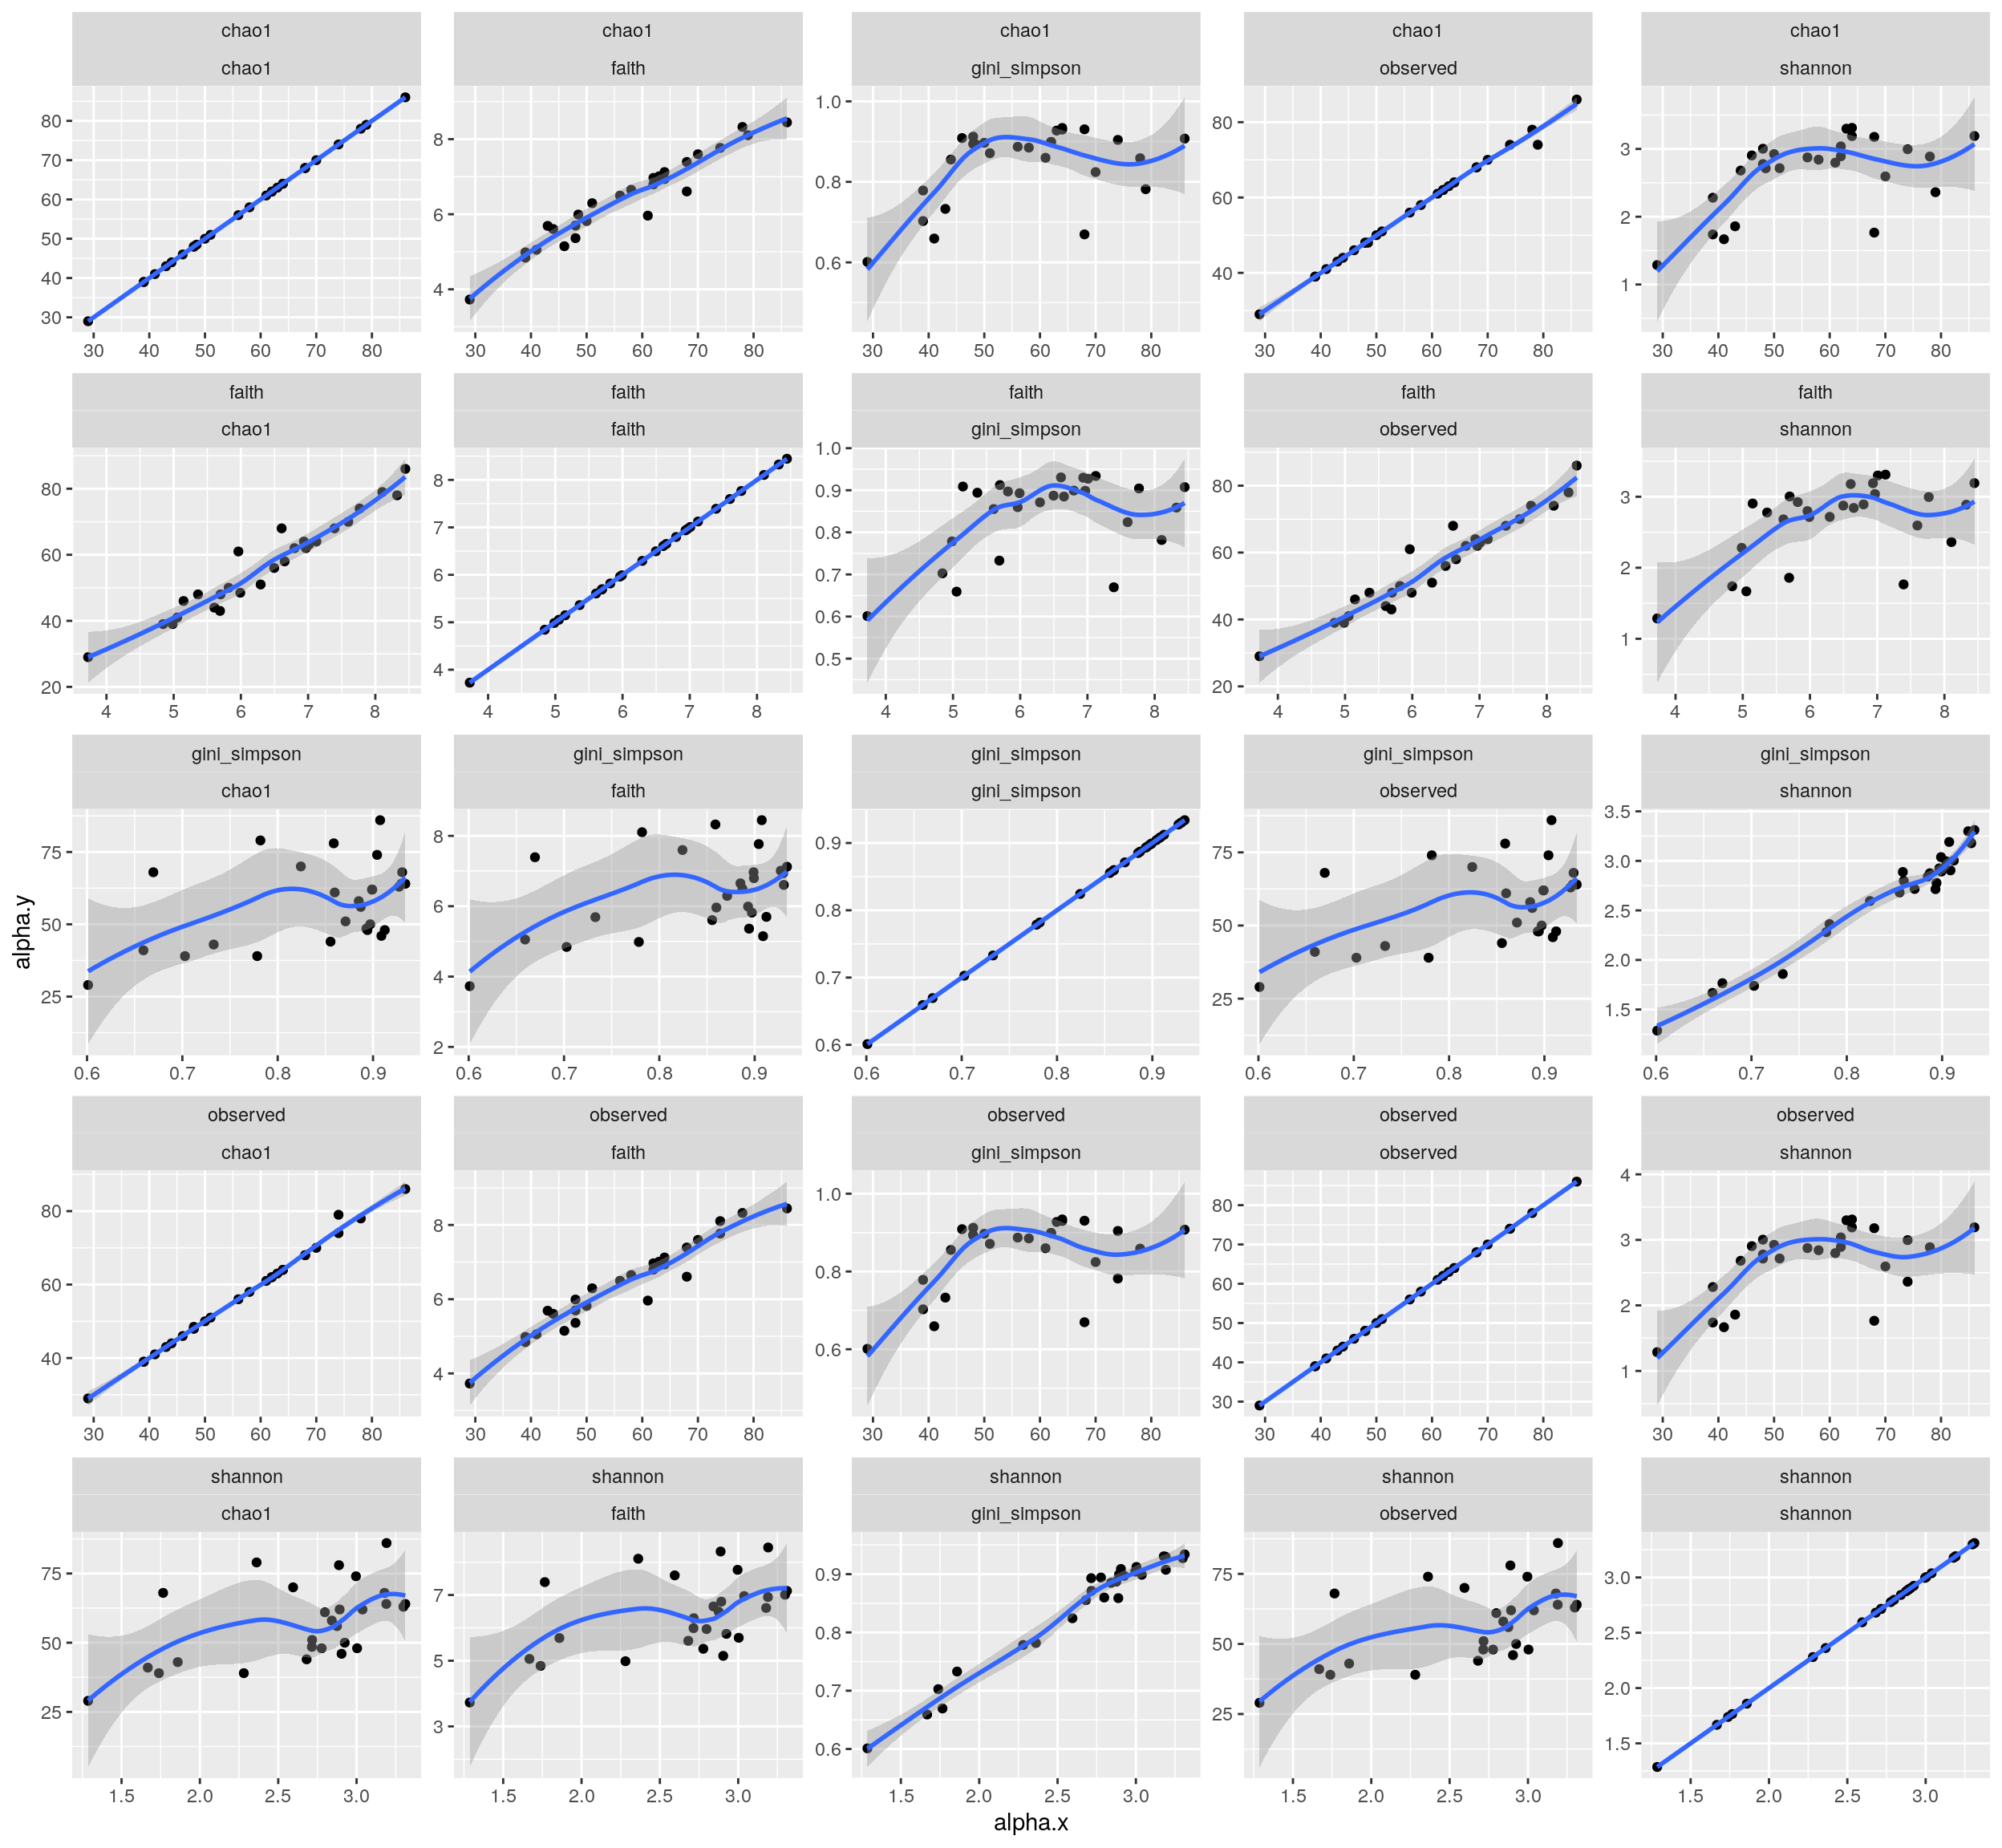
\includegraphics{05-alpha_diversity_demo_files/figure-latex/scatterlots-1.pdf}

\hypertarget{comparing-alpha-diversity}{%
\section{Comparing alpha diversity}\label{comparing-alpha-diversity}}

It is often interesting to look for any group differences:

\begin{Shaded}
\begin{Highlighting}[]
\NormalTok{p }\OtherTok{\textless{}{-}} \FunctionTok{as\_tibble}\NormalTok{(}\FunctionTok{colData}\NormalTok{(tse)) }\SpecialCharTok{\%\textgreater{}\%} 
  \FunctionTok{pivot\_longer}\NormalTok{(}\AttributeTok{cols =} \FunctionTok{c}\NormalTok{(}\StringTok{"shannon"}\NormalTok{,}\StringTok{"gini\_simpson"}\NormalTok{,}\StringTok{"faith"}\NormalTok{,}\StringTok{"chao1"}\NormalTok{,}\StringTok{"observed"}\NormalTok{), }\AttributeTok{names\_to =} \StringTok{"index"}\NormalTok{, }\AttributeTok{values\_to =} \StringTok{"alpha"}\NormalTok{) }\SpecialCharTok{\%\textgreater{}\%} 
  \FunctionTok{ggplot}\NormalTok{( }\FunctionTok{aes}\NormalTok{(}\AttributeTok{x =}\NormalTok{ patient\_status, }\AttributeTok{y =}\NormalTok{ alpha)) }\SpecialCharTok{+} 
  \FunctionTok{geom\_boxplot}\NormalTok{(}\AttributeTok{outlier.shape =} \ConstantTok{NA}\NormalTok{) }\SpecialCharTok{+}
  \FunctionTok{geom\_jitter}\NormalTok{(}\AttributeTok{alpha =}\FloatTok{0.5}\NormalTok{) }\SpecialCharTok{+}
  \FunctionTok{facet\_wrap}\NormalTok{(}\FunctionTok{vars}\NormalTok{(index), }\AttributeTok{scales =} \StringTok{"free"}\NormalTok{)}

\FunctionTok{print}\NormalTok{(p)}
\end{Highlighting}
\end{Shaded}

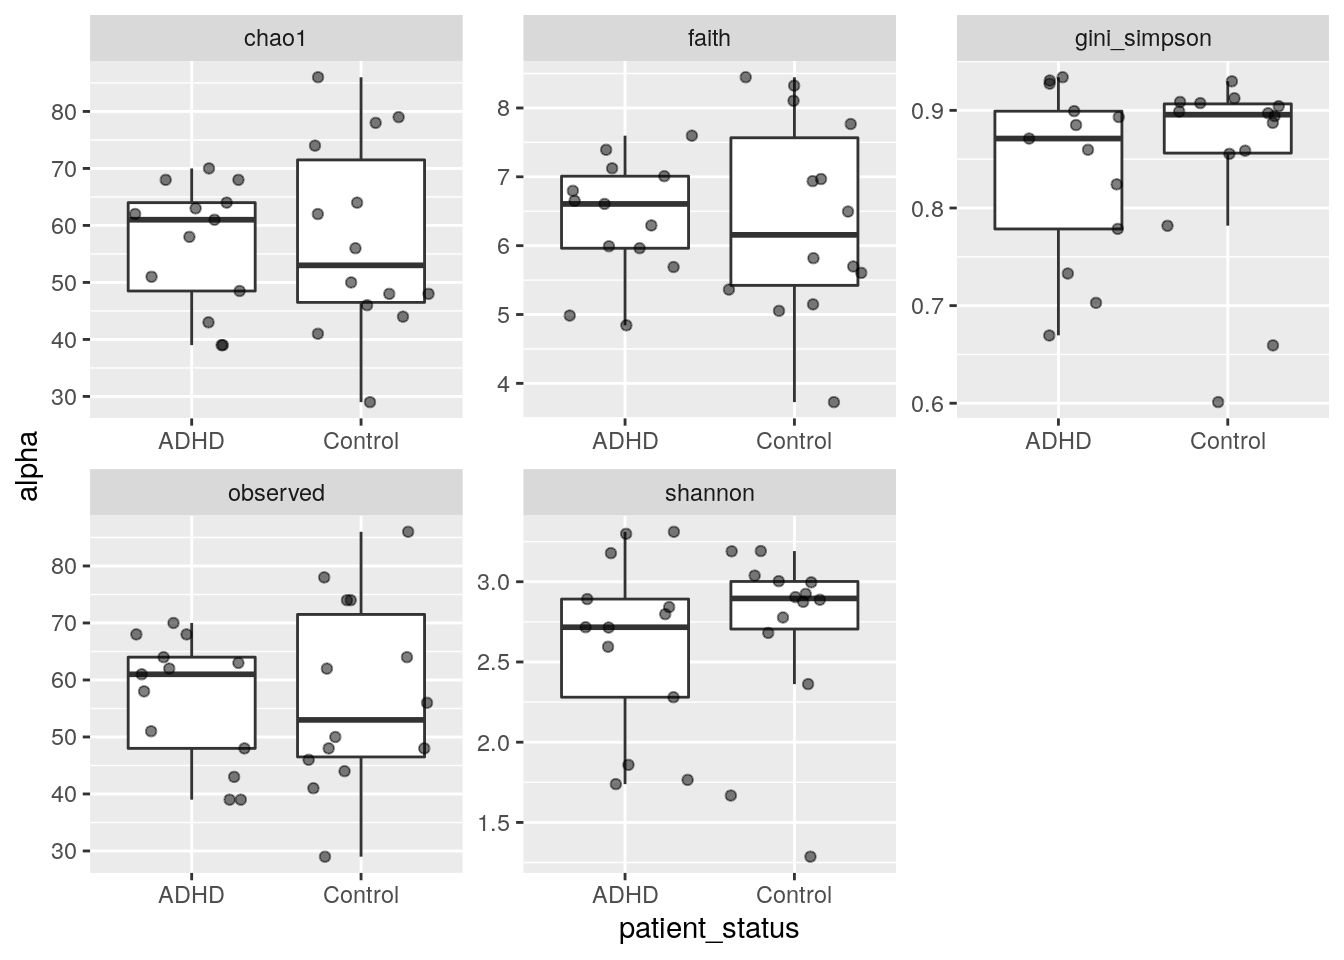
\includegraphics{05-alpha_diversity_demo_files/figure-latex/boxplots-1.pdf}

Moreover, we can test the group differences by parametric or non-parametric tests:

\begin{Shaded}
\begin{Highlighting}[]
\NormalTok{df1 }\OtherTok{\textless{}{-}} \FunctionTok{as\_tibble}\NormalTok{(}\FunctionTok{colData}\NormalTok{(tse)) }\SpecialCharTok{\%\textgreater{}\%} 
  \FunctionTok{pivot\_longer}\NormalTok{(}\AttributeTok{cols =} \FunctionTok{c}\NormalTok{(}\StringTok{"faith"}\NormalTok{,}\StringTok{"chao1"}\NormalTok{,}\StringTok{"observed"}\NormalTok{), }\AttributeTok{names\_to =} \StringTok{"index"}\NormalTok{, }\AttributeTok{values\_to =} \StringTok{"alpha"}\NormalTok{) }\SpecialCharTok{\%\textgreater{}\%} 
  \FunctionTok{group\_by}\NormalTok{(index) }\SpecialCharTok{\%\textgreater{}\%} 
  \FunctionTok{nest}\NormalTok{() }\SpecialCharTok{\%\textgreater{}\%} 
  \FunctionTok{mutate}\NormalTok{(}\AttributeTok{test\_pval =} \FunctionTok{map\_dbl}\NormalTok{(data, }\SpecialCharTok{\textasciitilde{}} \FunctionTok{t.test}\NormalTok{(alpha }\SpecialCharTok{\textasciitilde{}}\NormalTok{ patient\_status, }\AttributeTok{data =}\NormalTok{ .x)}\SpecialCharTok{$}\NormalTok{p.value)) }\SpecialCharTok{\%\textgreater{}\%} 
  \FunctionTok{mutate}\NormalTok{(}\AttributeTok{test =} \StringTok{"ttest"}\NormalTok{ ) }

\NormalTok{df2 }\OtherTok{\textless{}{-}} \FunctionTok{as\_tibble}\NormalTok{(}\FunctionTok{colData}\NormalTok{(tse)) }\SpecialCharTok{\%\textgreater{}\%} 
  \FunctionTok{pivot\_longer}\NormalTok{(}\AttributeTok{cols =} \FunctionTok{c}\NormalTok{(}\StringTok{"shannon"}\NormalTok{,}\StringTok{"gini\_simpson"}\NormalTok{), }\AttributeTok{names\_to =} \StringTok{"index"}\NormalTok{, }\AttributeTok{values\_to =} \StringTok{"alpha"}\NormalTok{) }\SpecialCharTok{\%\textgreater{}\%} 
  \FunctionTok{group\_by}\NormalTok{(index) }\SpecialCharTok{\%\textgreater{}\%} 
  \FunctionTok{nest}\NormalTok{() }\SpecialCharTok{\%\textgreater{}\%} 
  \FunctionTok{mutate}\NormalTok{(}\AttributeTok{test\_pval =} \FunctionTok{map\_dbl}\NormalTok{(data, }\SpecialCharTok{\textasciitilde{}} \FunctionTok{wilcox.test}\NormalTok{(alpha }\SpecialCharTok{\textasciitilde{}}\NormalTok{ patient\_status, }\AttributeTok{data =}\NormalTok{ .x)}\SpecialCharTok{$}\NormalTok{p.value))}\SpecialCharTok{\%\textgreater{}\%} 
  \FunctionTok{mutate}\NormalTok{(}\AttributeTok{test =} \StringTok{"wilcoxon"}\NormalTok{ ) }

\NormalTok{df }\OtherTok{\textless{}{-}} \FunctionTok{rbind}\NormalTok{(df1,df2) }\SpecialCharTok{\%\textgreater{}\%} \FunctionTok{select}\NormalTok{(}\SpecialCharTok{{-}}\NormalTok{data) }\SpecialCharTok{\%\textgreater{}\%} \FunctionTok{arrange}\NormalTok{(test\_pval) }\SpecialCharTok{\%\textgreater{}\%} \FunctionTok{ungroup}\NormalTok{()}

\NormalTok{df}
\end{Highlighting}
\end{Shaded}

\begin{verbatim}
## # A tibble: 5 x 3
##   index        test_pval test    
##   <chr>            <dbl> <chr>   
## 1 shannon          0.488 wilcoxon
## 2 gini_simpson     0.685 wilcoxon
## 3 chao1            0.856 ttest   
## 4 observed         0.900 ttest   
## 5 faith            0.983 ttest
\end{verbatim}

End of the demo.

\hypertarget{exercises}{%
\section{Exercises}\label{exercises}}

Do ``Alpha diversity basics'' from the \href{https://microbiome.github.io/OMA/exercises.html}{exercises}.

\hypertarget{beta-diversity-demo}{%
\chapter{Beta diversity demo}\label{beta-diversity-demo}}

\hypertarget{visualizations}{%
\section{Visualizations}\label{visualizations}}

Lets generate ordination plots with different methods and transformations.

\begin{Shaded}
\begin{Highlighting}[]
\DocumentationTok{\#\#\#\# calculating Bray Curtis dissimilarity and PCoA}

\NormalTok{tse }\OtherTok{\textless{}{-}} \FunctionTok{transformSamples}\NormalTok{(tse, }\AttributeTok{method =} \StringTok{"relabundance"}\NormalTok{)}
\NormalTok{tse }\OtherTok{\textless{}{-}} \FunctionTok{runMDS}\NormalTok{(tse, }\AttributeTok{FUN =}\NormalTok{ vegan}\SpecialCharTok{::}\NormalTok{vegdist, }\AttributeTok{method =} \StringTok{"bray"}\NormalTok{, }\AttributeTok{name =} \StringTok{"PCoA\_BC"}\NormalTok{, }\AttributeTok{exprs\_values =} \StringTok{"relabundance"}\NormalTok{)}


\NormalTok{p }\OtherTok{\textless{}{-}} \FunctionTok{plotReducedDim}\NormalTok{(tse, }\StringTok{"PCoA\_BC"}\NormalTok{, }\AttributeTok{colour\_by =} \StringTok{"patient\_status"}\NormalTok{)}

\CommentTok{\# Add explained variance for each axis}
\NormalTok{e }\OtherTok{\textless{}{-}} \FunctionTok{attr}\NormalTok{(}\FunctionTok{reducedDim}\NormalTok{(tse, }\StringTok{"PCoA\_BC"}\NormalTok{), }\StringTok{"eig"}\NormalTok{);}
\NormalTok{rel\_eig }\OtherTok{\textless{}{-}}\NormalTok{ e}\SpecialCharTok{/}\FunctionTok{sum}\NormalTok{(e[e}\SpecialCharTok{\textgreater{}}\DecValTok{0}\NormalTok{])          }
\NormalTok{p }\OtherTok{\textless{}{-}}\NormalTok{ p }\SpecialCharTok{+} \FunctionTok{labs}\NormalTok{(}\AttributeTok{x =} \FunctionTok{paste}\NormalTok{(}\StringTok{"PCoA 1 ("}\NormalTok{, }\FunctionTok{round}\NormalTok{(}\DecValTok{100} \SpecialCharTok{*}\NormalTok{ rel\_eig[[}\DecValTok{1}\NormalTok{]],}\DecValTok{1}\NormalTok{), }\StringTok{"\%"}\NormalTok{, }\StringTok{")"}\NormalTok{, }\AttributeTok{sep =} \StringTok{""}\NormalTok{),}
              \AttributeTok{y =} \FunctionTok{paste}\NormalTok{(}\StringTok{"PCoA 2 ("}\NormalTok{, }\FunctionTok{round}\NormalTok{(}\DecValTok{100} \SpecialCharTok{*}\NormalTok{ rel\_eig[[}\DecValTok{2}\NormalTok{]],}\DecValTok{1}\NormalTok{), }\StringTok{"\%"}\NormalTok{, }\StringTok{")"}\NormalTok{, }\AttributeTok{sep =} \StringTok{""}\NormalTok{))}

\FunctionTok{print}\NormalTok{(p)}
\end{Highlighting}
\end{Shaded}

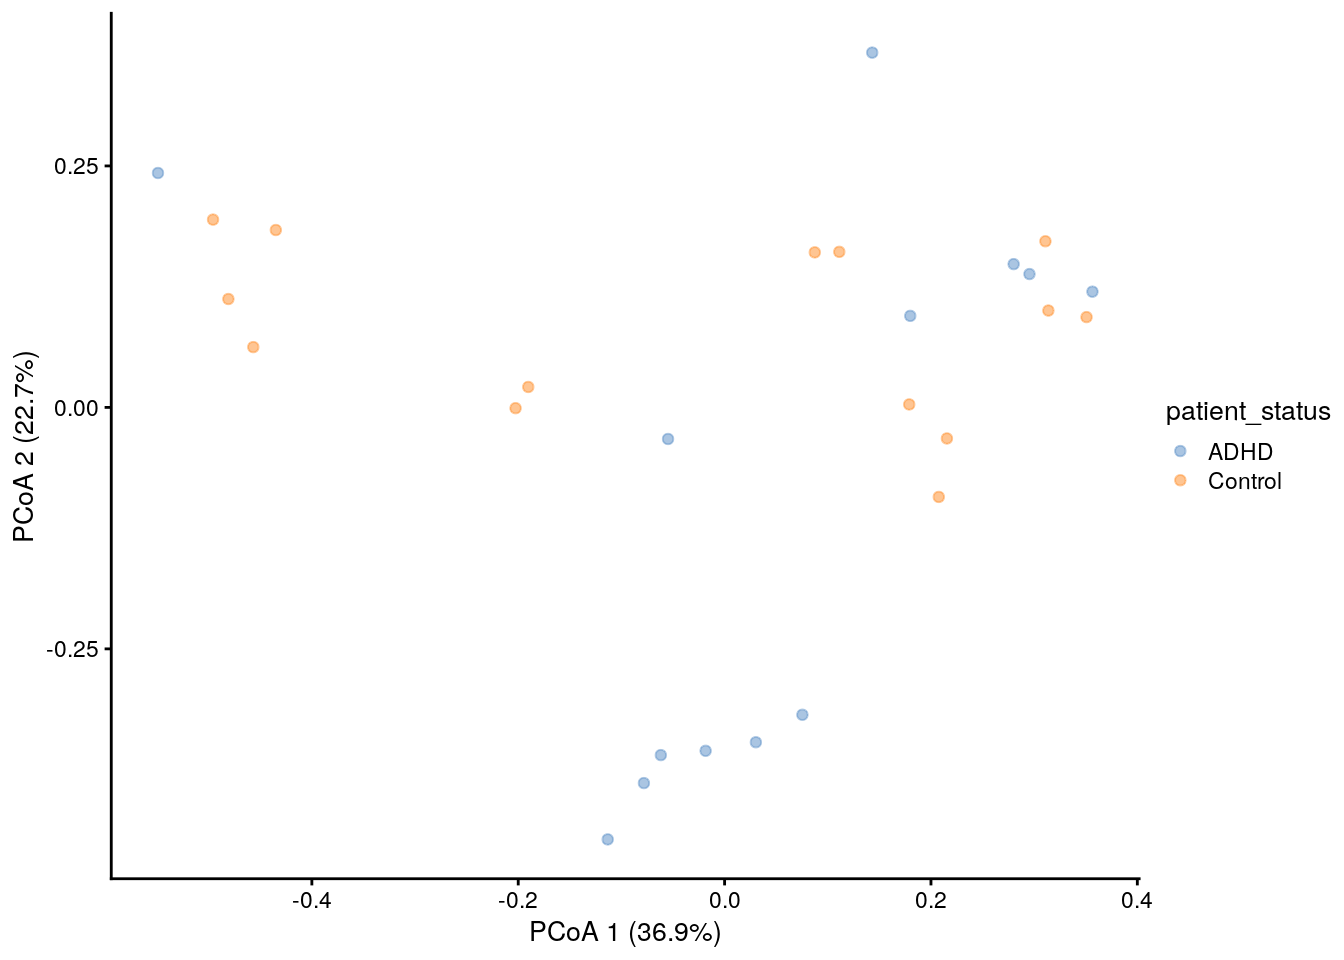
\includegraphics{06-beta_diversity_demo_files/figure-latex/viz1-1.pdf}

\begin{Shaded}
\begin{Highlighting}[]
\DocumentationTok{\#\#\#\# Aitchinson distances and PCA}

\NormalTok{tse }\OtherTok{\textless{}{-}} \FunctionTok{transformSamples}\NormalTok{(tse, }\AttributeTok{method =} \StringTok{"clr"}\NormalTok{, }\AttributeTok{pseudocount =} \DecValTok{1}\NormalTok{)}
\end{Highlighting}
\end{Shaded}

\begin{verbatim}
## Warning: All the total abundances of samples do not sum-up to a fixed constant.
## Please consider to apply, e.g., relative transformation in prior to CLR
## transformation.
\end{verbatim}

\begin{Shaded}
\begin{Highlighting}[]
\NormalTok{tse }\OtherTok{\textless{}{-}} \FunctionTok{runMDS}\NormalTok{(tse, }\AttributeTok{FUN =}\NormalTok{ vegan}\SpecialCharTok{::}\NormalTok{vegdist, }\AttributeTok{name =} \StringTok{"MDS\_euclidean"}\NormalTok{,}
              \AttributeTok{method =} \StringTok{"euclidean"}\NormalTok{, }\AttributeTok{exprs\_values =} \StringTok{"clr"}\NormalTok{)}

\NormalTok{p }\OtherTok{\textless{}{-}} \FunctionTok{plotReducedDim}\NormalTok{(tse, }\StringTok{"MDS\_euclidean"}\NormalTok{, }\AttributeTok{colour\_by =} \StringTok{"patient\_status\_vs\_cohort"}\NormalTok{)}

\CommentTok{\# Add explained variance for each axis}
\NormalTok{e }\OtherTok{\textless{}{-}} \FunctionTok{attr}\NormalTok{(}\FunctionTok{reducedDim}\NormalTok{(tse, }\StringTok{"MDS\_euclidean"}\NormalTok{), }\StringTok{"eig"}\NormalTok{);}
\NormalTok{rel\_eig }\OtherTok{\textless{}{-}}\NormalTok{ e}\SpecialCharTok{/}\FunctionTok{sum}\NormalTok{(e[e}\SpecialCharTok{\textgreater{}}\DecValTok{0}\NormalTok{])          }
\NormalTok{p }\OtherTok{\textless{}{-}}\NormalTok{ p }\SpecialCharTok{+} \FunctionTok{labs}\NormalTok{(}\AttributeTok{x =} \FunctionTok{paste}\NormalTok{(}\StringTok{"Axis 1 ("}\NormalTok{, }\FunctionTok{round}\NormalTok{(}\DecValTok{100} \SpecialCharTok{*}\NormalTok{ rel\_eig[[}\DecValTok{1}\NormalTok{]],}\DecValTok{1}\NormalTok{), }\StringTok{"\%"}\NormalTok{, }\StringTok{")"}\NormalTok{, }\AttributeTok{sep =} \StringTok{""}\NormalTok{),}
              \AttributeTok{y =} \FunctionTok{paste}\NormalTok{(}\StringTok{"Axis 2 ("}\NormalTok{, }\FunctionTok{round}\NormalTok{(}\DecValTok{100} \SpecialCharTok{*}\NormalTok{ rel\_eig[[}\DecValTok{2}\NormalTok{]],}\DecValTok{1}\NormalTok{), }\StringTok{"\%"}\NormalTok{, }\StringTok{")"}\NormalTok{, }\AttributeTok{sep =} \StringTok{""}\NormalTok{))}

\FunctionTok{print}\NormalTok{(p)}
\end{Highlighting}
\end{Shaded}

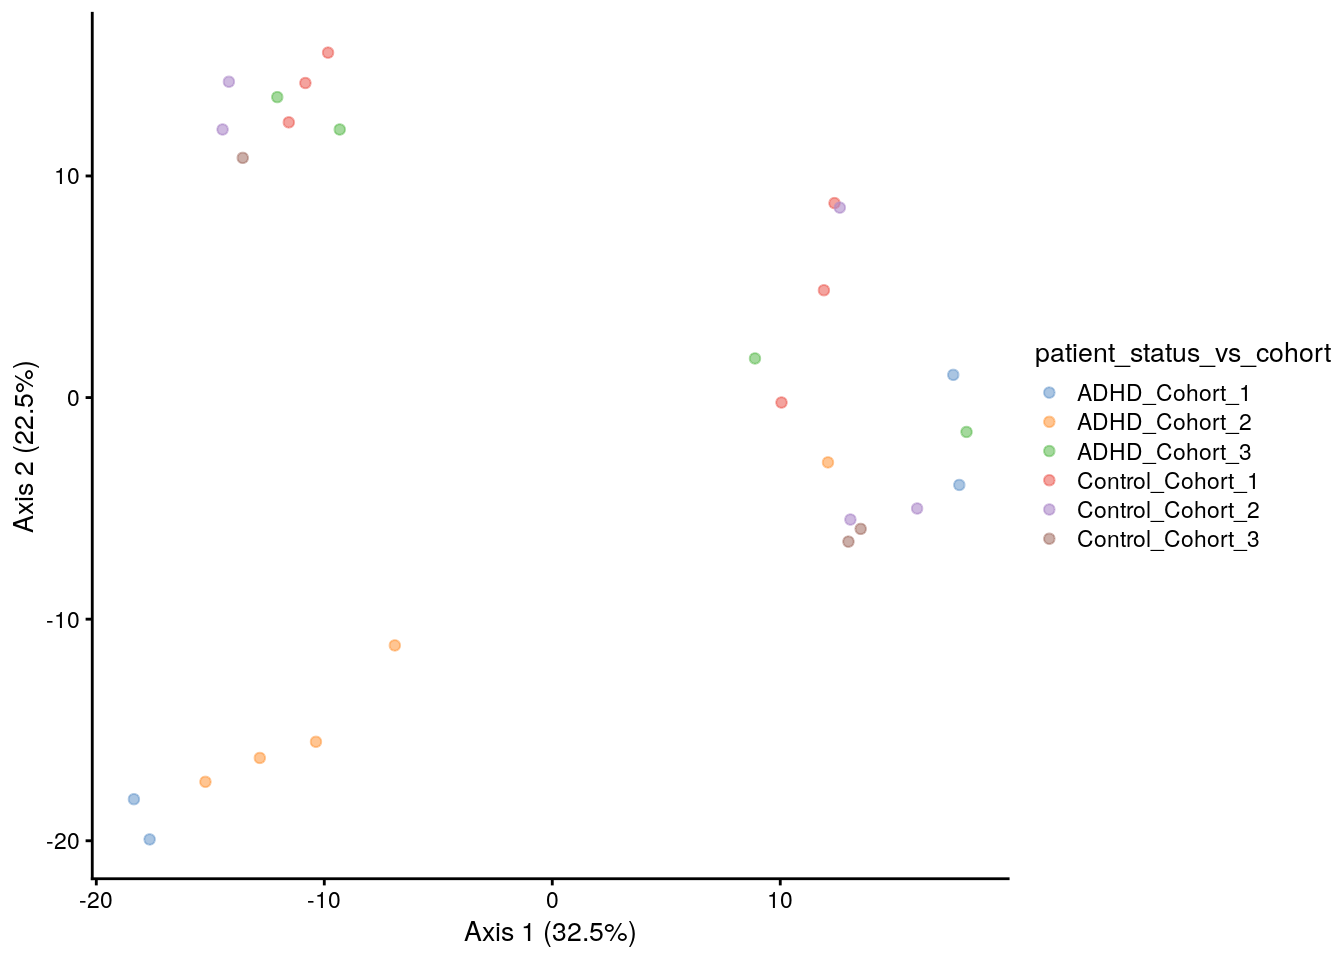
\includegraphics{06-beta_diversity_demo_files/figure-latex/viz1-2.pdf}

PCA is a subtype of MDS with Euclidean distances, below is a different alternative for running the same analysis.

\begin{Shaded}
\begin{Highlighting}[]
\CommentTok{\# alternative method }

\NormalTok{tse }\OtherTok{\textless{}{-}} \FunctionTok{runPCA}\NormalTok{(tse, }\AttributeTok{name =} \StringTok{"PCA"}\NormalTok{, }\AttributeTok{exprs\_values =} \StringTok{"clr"}\NormalTok{, }\AttributeTok{ncomponents =} \DecValTok{10}\NormalTok{)}
\FunctionTok{plotReducedDim}\NormalTok{(tse, }\StringTok{"PCA"}\NormalTok{, }\AttributeTok{colour\_by =} \StringTok{"patient\_status\_vs\_cohort"}\NormalTok{)}
\end{Highlighting}
\end{Shaded}

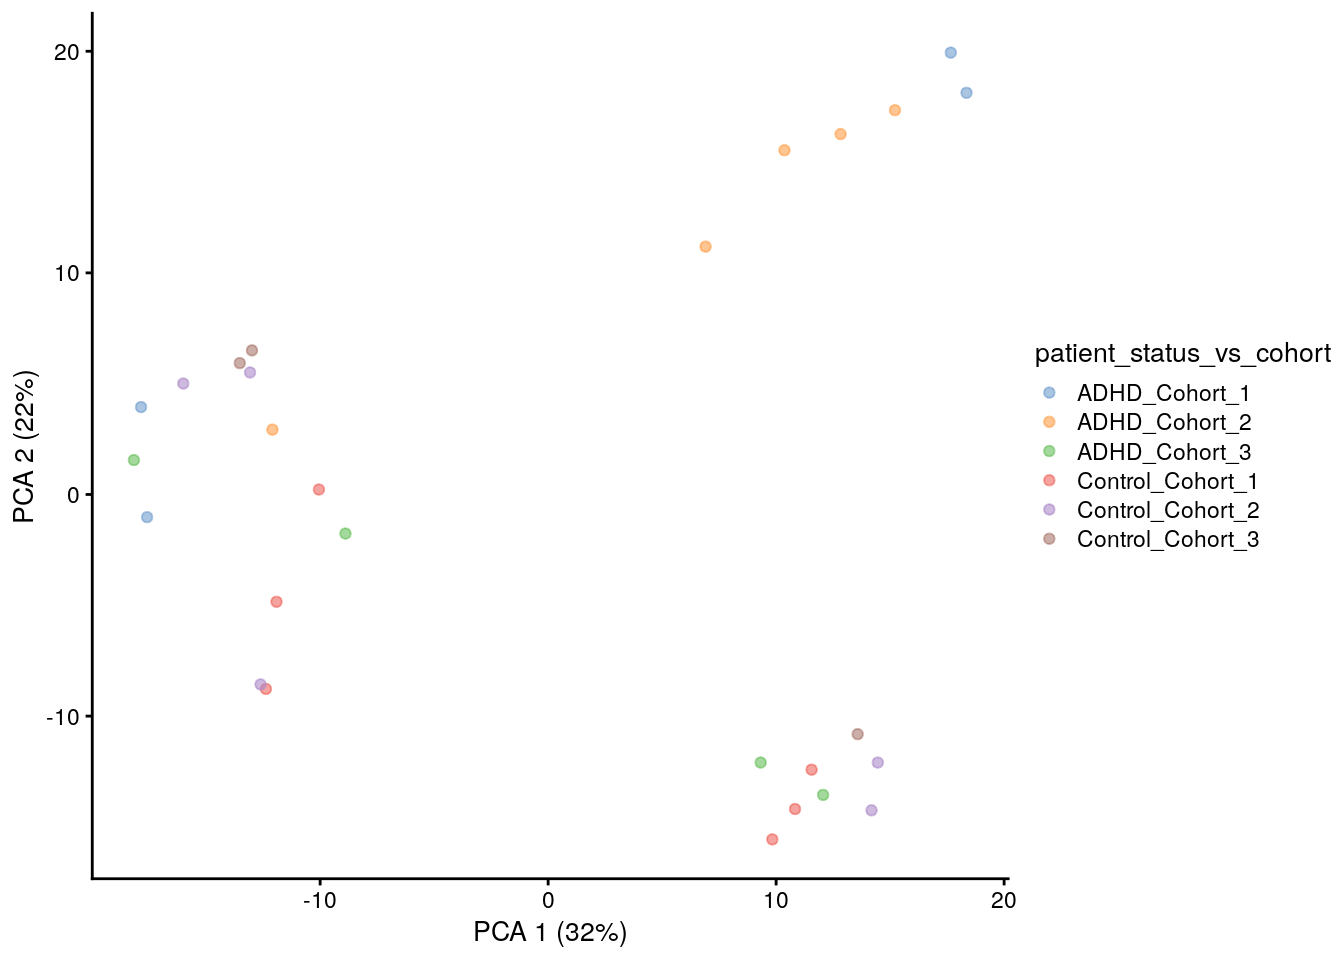
\includegraphics{06-beta_diversity_demo_files/figure-latex/viz2-1.pdf}

One can use also ggplot for ordination plots for the flexible adaptablity.

\begin{Shaded}
\begin{Highlighting}[]
\NormalTok{dis }\OtherTok{\textless{}{-}}\NormalTok{ vegan}\SpecialCharTok{::}\FunctionTok{vegdist}\NormalTok{(}\FunctionTok{t}\NormalTok{(}\FunctionTok{assays}\NormalTok{(tse)}\SpecialCharTok{$}\NormalTok{counts), }\AttributeTok{method =} \StringTok{"jaccard"}\NormalTok{)}

\CommentTok{\# principal coordinate analysis}
\NormalTok{jaccard\_pcoa }\OtherTok{\textless{}{-}}\NormalTok{ ecodist}\SpecialCharTok{::}\FunctionTok{pco}\NormalTok{(dis)}

\CommentTok{\# a data frame from principal coordinates and groupng variable}
\NormalTok{jaccard\_pcoa\_df }\OtherTok{\textless{}{-}} \FunctionTok{data.frame}\NormalTok{(}\AttributeTok{pcoa1 =}\NormalTok{ jaccard\_pcoa}\SpecialCharTok{$}\NormalTok{vectors[,}\DecValTok{1}\NormalTok{], }
                                \AttributeTok{pcoa2 =}\NormalTok{ jaccard\_pcoa}\SpecialCharTok{$}\NormalTok{vectors[,}\DecValTok{2}\NormalTok{],}
                              \AttributeTok{patient\_status\_vs\_cohort =}  \FunctionTok{colData}\NormalTok{(tse)}\SpecialCharTok{$}\NormalTok{patient\_status\_vs\_cohort)}


\CommentTok{\# plot}
\NormalTok{jaccard\_plot }\OtherTok{\textless{}{-}} \FunctionTok{ggplot}\NormalTok{(}\AttributeTok{data =}\NormalTok{ jaccard\_pcoa\_df, }\FunctionTok{aes}\NormalTok{(}\AttributeTok{x=}\NormalTok{pcoa1, }\AttributeTok{y=}\NormalTok{pcoa2, }\AttributeTok{color =}\NormalTok{ patient\_status\_vs\_cohort)) }\SpecialCharTok{+}
  \FunctionTok{geom\_point}\NormalTok{() }\SpecialCharTok{+}
  \FunctionTok{labs}\NormalTok{(}\AttributeTok{x =} \FunctionTok{paste}\NormalTok{(}\StringTok{"Axis 1 ("}\NormalTok{, }\FunctionTok{round}\NormalTok{(}\DecValTok{100} \SpecialCharTok{*}\NormalTok{ jaccard\_pcoa}\SpecialCharTok{$}\NormalTok{values[[}\DecValTok{1}\NormalTok{]] }\SpecialCharTok{/} \FunctionTok{sum}\NormalTok{(jaccard\_pcoa}\SpecialCharTok{$}\NormalTok{values), }\DecValTok{1}\NormalTok{), }\StringTok{"\%"}\NormalTok{, }\StringTok{")"}\NormalTok{, }\AttributeTok{sep =} \StringTok{""}\NormalTok{),}
       \AttributeTok{y =} \FunctionTok{paste}\NormalTok{(}\StringTok{"Axis 2 ("}\NormalTok{, }\FunctionTok{round}\NormalTok{(}\DecValTok{100} \SpecialCharTok{*}\NormalTok{ jaccard\_pcoa}\SpecialCharTok{$}\NormalTok{values[[}\DecValTok{2}\NormalTok{]] }\SpecialCharTok{/} \FunctionTok{sum}\NormalTok{(jaccard\_pcoa}\SpecialCharTok{$}\NormalTok{values), }\DecValTok{1}\NormalTok{), }\StringTok{"\%"}\NormalTok{, }\StringTok{")"}\NormalTok{, }\AttributeTok{sep =} \StringTok{""}\NormalTok{),}
       \AttributeTok{title =} \StringTok{"Jaccard PCoA"}\NormalTok{) }\SpecialCharTok{+}
  \FunctionTok{theme}\NormalTok{(}\AttributeTok{title =} \FunctionTok{element\_text}\NormalTok{(}\AttributeTok{size =} \DecValTok{12}\NormalTok{)) }\SpecialCharTok{+}
  \FunctionTok{theme\_light}\NormalTok{()}

\NormalTok{jaccard\_plot}
\end{Highlighting}
\end{Shaded}

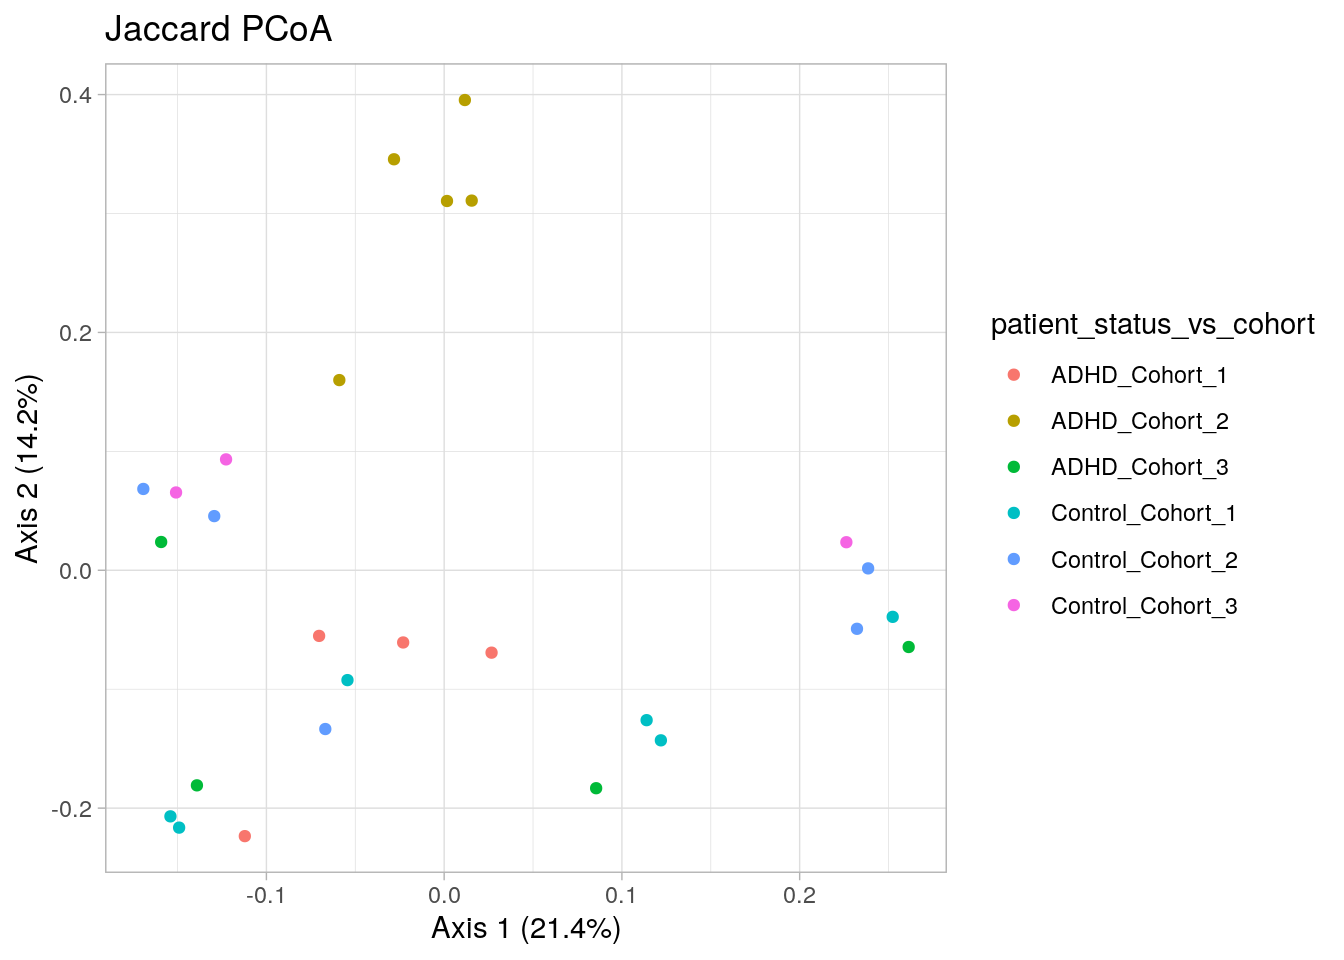
\includegraphics{06-beta_diversity_demo_files/figure-latex/viz ggplot-1.pdf}

\hypertarget{hypothesis-testing}{%
\section{Hypothesis testing}\label{hypothesis-testing}}

PERMANOVA with the function adonis is most commonly used to detect differences in multivariate data.
adonis function was recently updated with slightly different functionality. Now the adonis2 allows independent analysis of terms.

\begin{Shaded}
\begin{Highlighting}[]
\NormalTok{variable\_names }\OtherTok{\textless{}{-}} \FunctionTok{c}\NormalTok{(}\StringTok{"patient\_status"}\NormalTok{, }\StringTok{"cohort"}\NormalTok{)}

\NormalTok{tse\_genus }\OtherTok{\textless{}{-}} \FunctionTok{agglomerateByRank}\NormalTok{(tse, }\StringTok{"Genus"}\NormalTok{)}
\end{Highlighting}
\end{Shaded}

\begin{verbatim}
## Warning: 'clr' includes negative values.
## Agglomeration of it might lead to meaningless values.
## Check the assay, and consider doing transformation again manually with agglomerated data.
\end{verbatim}

\begin{Shaded}
\begin{Highlighting}[]
\CommentTok{\# Apply relative transform}
\NormalTok{tse\_genus }\OtherTok{\textless{}{-}} \FunctionTok{transformSamples}\NormalTok{(tse\_genus, }\AttributeTok{method =} \StringTok{"relabundance"}\NormalTok{)}


\FunctionTok{set.seed}\NormalTok{(}\DecValTok{12346}\NormalTok{)}
\CommentTok{\# We choose 99 random permutations for speed. Consider applying more (999 or 9999) }

\NormalTok{assay }\OtherTok{\textless{}{-}} \FunctionTok{t}\NormalTok{(}\FunctionTok{assay}\NormalTok{(tse\_genus,}\StringTok{"relabundance"}\NormalTok{))}

\NormalTok{mod }\OtherTok{\textless{}{-}} \FunctionTok{paste}\NormalTok{(}\StringTok{"assay \textasciitilde{}"}\NormalTok{, }\FunctionTok{paste}\NormalTok{(variable\_names, }\AttributeTok{collapse=}\StringTok{"+"}\NormalTok{)) }\SpecialCharTok{\%\textgreater{}\%} \FunctionTok{as.formula}\NormalTok{()}

\NormalTok{permanova2 }\OtherTok{\textless{}{-}}\NormalTok{ vegan}\SpecialCharTok{::}\FunctionTok{adonis2}\NormalTok{(mod,}
                     \AttributeTok{by =} \StringTok{"margin"}\NormalTok{, }\CommentTok{\# each term analyzed individually}
                     \AttributeTok{data =} \FunctionTok{colData}\NormalTok{(tse),}
                     \AttributeTok{method =} \StringTok{"bray"}\NormalTok{,}
                     \AttributeTok{permutations =} \DecValTok{99}\NormalTok{)}

\FunctionTok{print}\NormalTok{(permanova2)}
\end{Highlighting}
\end{Shaded}

\begin{verbatim}
## Permutation test for adonis under reduced model
## Marginal effects of terms
## Permutation: free
## Number of permutations: 99
## 
## vegan::adonis2(formula = mod, data = colData(tse), permutations = 99, method = "bray", by = "margin")
##                Df SumOfSqs      R2     F Pr(>F)
## patient_status  1   0.1885 0.05817 1.490   0.23
## cohort          2   0.1450 0.04474 0.573   0.75
## Residual       23   2.9104 0.89787             
## Total          26   3.2414 1.00000
\end{verbatim}

\begin{Shaded}
\begin{Highlighting}[]
\CommentTok{\# older adonis for reference}
\NormalTok{permanova }\OtherTok{\textless{}{-}}\NormalTok{ vegan}\SpecialCharTok{::}\FunctionTok{adonis}\NormalTok{(mod,}
                            \CommentTok{\#by = "margin", \# each term analyzed sequentially}
                            \AttributeTok{data =} \FunctionTok{colData}\NormalTok{(tse),}
                            \AttributeTok{method =} \StringTok{"bray"}\NormalTok{,}
                            \AttributeTok{permutations =} \DecValTok{99}\NormalTok{)}
\end{Highlighting}
\end{Shaded}

\begin{verbatim}
## 'adonis' will be deprecated: use 'adonis2' instead
\end{verbatim}

\begin{Shaded}
\begin{Highlighting}[]
\NormalTok{permanova}\SpecialCharTok{$}\NormalTok{aov.tab}
\end{Highlighting}
\end{Shaded}

\begin{verbatim}
## Permutation: free
## Number of permutations: 99
## 
## Terms added sequentially (first to last)
## 
##                Df SumsOfSqs  MeanSqs F.Model      R2 Pr(>F)
## patient_status  1    0.1860 0.186024 1.47011 0.05739   0.22
## cohort          2    0.1450 0.072503 0.57298 0.04474   0.79
## Residuals      23    2.9104 0.126537         0.89787       
## Total          26    3.2414                  1.00000
\end{verbatim}

With older adonis version one cam calculate top coefficients driving the differences between groups.

\begin{Shaded}
\begin{Highlighting}[]
\CommentTok{\# older adonis supplies the coefficients}
\NormalTok{coef }\OtherTok{\textless{}{-}} \FunctionTok{coefficients}\NormalTok{(permanova)[}\StringTok{"cohort1"}\NormalTok{,]}
\NormalTok{top.coef }\OtherTok{\textless{}{-}} \FunctionTok{sort}\NormalTok{(}\FunctionTok{head}\NormalTok{(coef[}\FunctionTok{rev}\NormalTok{(}\FunctionTok{order}\NormalTok{(}\FunctionTok{abs}\NormalTok{(coef)))],}\DecValTok{20}\NormalTok{))}

\CommentTok{\# plot }
\NormalTok{top\_taxa\_coeffient\_plot }\OtherTok{\textless{}{-}} \FunctionTok{ggplot}\NormalTok{(}\FunctionTok{data.frame}\NormalTok{(}\AttributeTok{x =}\NormalTok{ top.coef,}
                                             \AttributeTok{y =} \FunctionTok{factor}\NormalTok{(}\FunctionTok{names}\NormalTok{(top.coef),}
                                                        \FunctionTok{unique}\NormalTok{(}\FunctionTok{names}\NormalTok{(top.coef)))),}
                                  \FunctionTok{aes}\NormalTok{(}\AttributeTok{x =}\NormalTok{ x, }\AttributeTok{y =}\NormalTok{ y)) }\SpecialCharTok{+}
  \FunctionTok{geom\_bar}\NormalTok{(}\AttributeTok{stat=}\StringTok{"identity"}\NormalTok{) }\SpecialCharTok{+}
  \FunctionTok{labs}\NormalTok{(}\AttributeTok{x=}\StringTok{""}\NormalTok{, }\AttributeTok{y=}\StringTok{""}\NormalTok{, }\AttributeTok{title=}\StringTok{"Top Taxa"}\NormalTok{) }\SpecialCharTok{+}
  \FunctionTok{theme\_bw}\NormalTok{()}

\NormalTok{top\_taxa\_coeffient\_plot}
\end{Highlighting}
\end{Shaded}

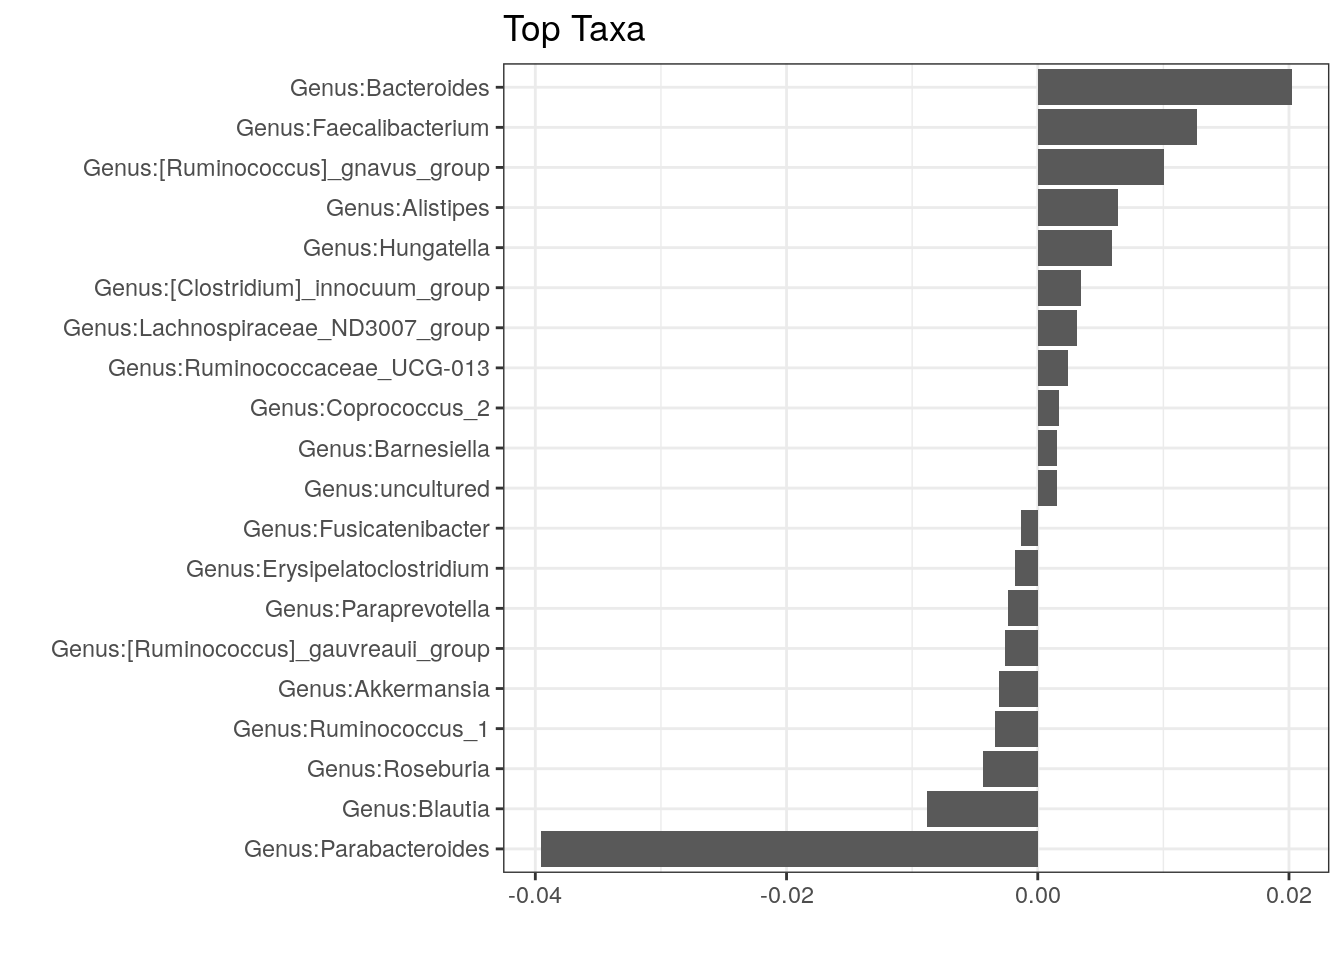
\includegraphics{06-beta_diversity_demo_files/figure-latex/permanova coef-1.pdf}

\hypertarget{testing-the-differences-in-dispersion}{%
\subsection{Testing the differences in dispersion}\label{testing-the-differences-in-dispersion}}

PEMRANOVA doesn't differentiate between different within-group variation, i.e.~dispersion, or the mean differences between groups, i.e.~the location of the centroid.
Follow-up testing can be done with PERMDISP2 implemented in the vegan package.

\begin{Shaded}
\begin{Highlighting}[]
\NormalTok{dis }\OtherTok{\textless{}{-}}\NormalTok{ vegan}\SpecialCharTok{::}\FunctionTok{vegdist}\NormalTok{(}\FunctionTok{t}\NormalTok{(}\FunctionTok{assays}\NormalTok{(tse)}\SpecialCharTok{$}\NormalTok{counts), }\AttributeTok{method =} \StringTok{"bray"}\NormalTok{)}
\NormalTok{b }\OtherTok{\textless{}{-}}\NormalTok{ vegan}\SpecialCharTok{::}\FunctionTok{betadisper}\NormalTok{(dis, }\FunctionTok{colData}\NormalTok{(tse)}\SpecialCharTok{$}\NormalTok{cohort)}
\FunctionTok{print}\NormalTok{(}\FunctionTok{anova}\NormalTok{(b))}
\end{Highlighting}
\end{Shaded}

\begin{verbatim}
## Analysis of Variance Table
## 
## Response: Distances
##           Df   Sum Sq   Mean Sq F value Pr(>F)
## Groups     2 0.000375 0.0001875  0.0166 0.9835
## Residuals 24 0.270795 0.0112831
\end{verbatim}

\begin{Shaded}
\begin{Highlighting}[]
\CommentTok{\# boxplor for distances to centroid}
\NormalTok{p }\OtherTok{\textless{}{-}} \FunctionTok{cbind}\NormalTok{(}\AttributeTok{distance =} \FunctionTok{as.numeric}\NormalTok{(b}\SpecialCharTok{$}\NormalTok{distances),}
          \AttributeTok{cohort =} \FunctionTok{colData}\NormalTok{(tse)}\SpecialCharTok{$}\NormalTok{cohort) }\SpecialCharTok{\%\textgreater{}\%} 
  \FunctionTok{as\_tibble}\NormalTok{() }\SpecialCharTok{\%\textgreater{}\%} 
  \FunctionTok{mutate}\NormalTok{(}\AttributeTok{distance =} \FunctionTok{as.numeric}\NormalTok{(distance)) }\SpecialCharTok{\%\textgreater{}\%} 
  \FunctionTok{ggplot}\NormalTok{(}\FunctionTok{aes}\NormalTok{(cohort, distance)) }\SpecialCharTok{+} 
  \FunctionTok{geom\_boxplot}\NormalTok{() }\SpecialCharTok{+}
  \FunctionTok{theme\_light}\NormalTok{()}

\FunctionTok{print}\NormalTok{(p)}
\end{Highlighting}
\end{Shaded}

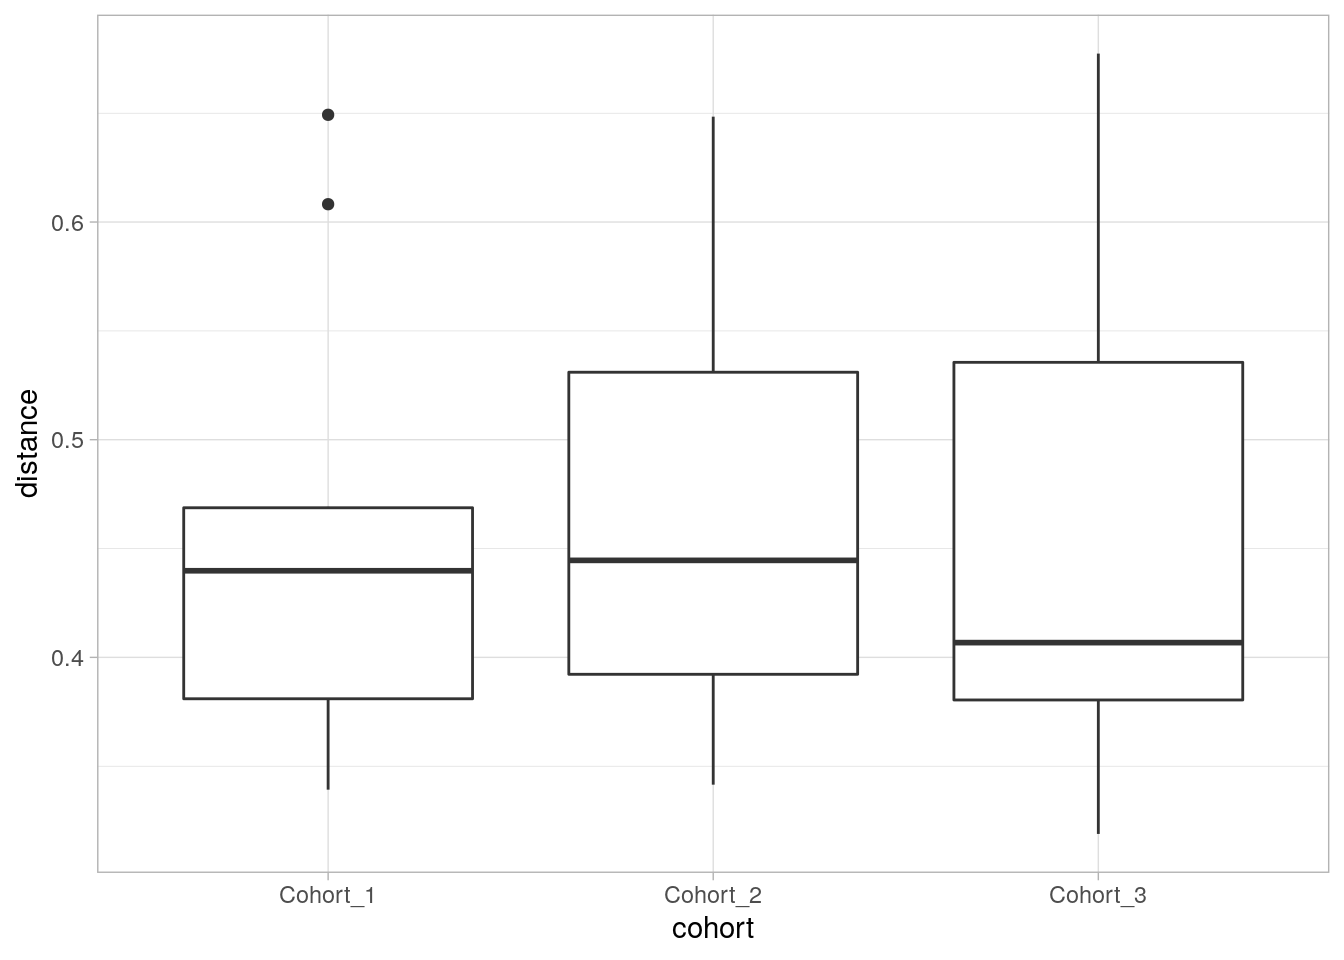
\includegraphics{06-beta_diversity_demo_files/figure-latex/dispersion-1.pdf}

End of the demo.

\hypertarget{exercises-1}{%
\section{Exercises}\label{exercises-1}}

Do ``Beta diversity'' from the \href{https://microbiome.github.io/OMA/exercises.html}{exercises}.

  \bibliography{packages.bib}

\end{document}
